\chapter{人类前额叶皮层:从指令和想像中产生目标} \label{chap:chap9}

这本书提出了关于灵长类动物前额叶皮层基本功能的方案。


\section{概述}

本章的目的是:检验我们关于前额叶皮层基本功能的建议是否可以解释当人们执行复杂认知任务时在那里发生的成像激活。
人类前额叶皮层中的许多激活似乎反映了对背景、目标和结果层次结构的阐述,从背景中生成目标,使用事件和抽象规则来选择目标,或目标的前瞻性编码。
其中一些激活发生在可能出现在类人猿或人类进化过程中的区域中,我们试图通过重新表示这一概念来解释这些。
现有前额叶皮层的扩展以及新区域的可能出现,导致人脑的大小和形状发生变化,连接方式也发生变化。
我们提出了一个观点:现代人和猴子的前额叶皮层执行从他们最后的共同祖先继承的共同功能:
它以减少错误的方式产生目标。
在一个关键的进化过程中,人类前额叶皮层进一步减少了错误,因为人们可以从指令或模仿中学习,并且因为人们可以在采取任何行动之前进行心理试错行为。
得出结论:人类可能可以完全避免错误。



\section{介绍}

第\ref{chap:chap8}章提出前额叶皮层具有简单的基本功能。
本章探讨该功能是否可以解释在受试者执行复杂认知任务时在人类前额叶皮层中看到的成像激活。
\par


读者会体会到我们这项工作的艰巨性。
我们在第\ref{chap:chap8}章中提出的建议在很大程度上取决于来自猴子的数据。
这些数据主要涉及地点和物体之间的选择,如通过伸手或眼球移动来实现的。
说这些功能与类比推理或做出道德判断相去甚远,至少可以说是一种轻描淡写的说法。
\par


这个问题类似于奥基夫和纳德尔(1978)首次提出海马体具有导航功能时所面临的问题。
当时,导航机制如何支持情景记忆似乎还是个谜,尽管从那时起,这种组合就变得不那么神秘了(市政厅,2002)。
我们现在可以理解海马体在导航中的祖先作用如何在进化过程中得到详细阐述,以涵盖复杂的认知功能,如情景记忆。
同样,本章试图根据为做出更好的觅食选择而进化的祖先机制的阐述来解释复杂认知任务的激活(第\ref{chap:chap8}章)。
\par


有足够的时间来详细说明。
只需考虑一个事实,即旧大陆猴子和人类的最后一个共同祖先生活在23万年或更久以前((凯等人,2004年;库马尔等人,2005年)。
这个事实意味着这两个世系已经分别进化了数千万年,在那段时间里,人类和猴子的大脑肯定都发生了变化。
在此期间,人类的大脑变得比同样体重的猴子预期的大4.8倍(麦克劳德等人,2003年)。
与此同时,人脑发展出了自己的专业化,这在整本书中都有评论。
\par


本章首先简要总结了人类大脑在进化过程中大小和形状的变化,重点是颗粒状前额叶皮层。
然后它处理连接和组织,包括新区域的可能出现。
本章的其余部分解决了关键问题:第 \ref{chap:chap8} 章为类人前脑皮层提出的简单功能能否解释高级认知期间人类前脑皮层中发生的成像激活?



\section{人类进化中的额叶}

遗传证据表明,类人猿在5-7Ma(库马尔等人,2005年)与人类世系分道扬镳,而最早的化石可能是原始人乍得沙赫人(盖等人,2005年),其年代约为7Ma(乐福等人,2009年)。
这种灵长类动物的颅骨容量约为360–370cm3,与小黑猩猩大致相同(居耶塔尔,2005)。
现代人脑平均约为1350–1550立方厘米(索韦尔塔尔,2007)。
当然,人往往比黑猩猩大,但我们的大脑仍然比相同体型的假想类人猿的大脑大3.5倍(麦克劳德等人,2003年)。
\par



所以原始人的大脑开始时很小,至少以现代人类的标准来看是这样。
这段历史类似于第\ref{chap:chap2}章为类人猿大脑描绘的历史:
在其早期进化历史中,大脑相对于身体尺寸而言相对较小,随后在其后期进化过程中大脑尺寸出现“等级增加”。
不幸的是,我们无法测量化石原始人额叶的大小。
与第\ref{chap:chap2}章描述的化石类人猿大脑不同,人科动物硬脑膜的厚度阻止了在其头骨内表面形成清晰的脑沟印迹。
所以我们只能评论大脑的整体形状。
由此,我们知道在原始人进化过程中,前额叶变得更宽、更圆。
\par


福尔克等人(2000)制作了纤细而健壮的南方古猿的内脑模型,早期原始人的寿命约为1.5–2.5Ma。
在“健壮”的南方古猿旁人属中,额叶具有相对尖的形状,类似于现代黑猩猩和大猩猩。
在细长的南方古猿中,额叶的形状略微更圆。
我们很幸运有一个保存完好的南方古猿的头骨,它来自南非,年代约为2Ma(卡尔索内塔尔,2011)。
眶额皮层和额极皮层的形状表明向更圆的形式过渡似乎在人属的原始人中。
\par


布鲁纳和霍洛威(2010)测量了南方古猿额叶的最大宽度,并将这一结果与直立人和尼安德特人这两种后来进化的原始人的宽度进行了比较。
相对于内脑的最大宽度,更晚近的原始人的额叶宽度超过了南方古猿。
这一发现表明,在原始人类进化过程中,额叶的相对大小有所增加。
\par


现代人类可能是从与海德堡人有亲缘关系的原始人进化而来,有时也被称为古人类。
来自埃塞俄比亚60万年前(Ka)的博多头骨和来自赞比亚300Ka的卡布韦头骨来自这个物种。
布克斯坦等人(1999)测量了这些头骨中大脑内壳前部的斜率,并将其与早期现代人类的两个头骨的斜率进行了比较:
来自埃塞俄比亚的OmoI和OmoII头骨,日期为195Ka(1969年)。
尽管古代人类头骨与早期现代人的头骨不同,眉骨较大,但内额脑壳的倾斜度并无不同。
这一发现表明额叶的形状在古代人类中达到了现代状态,~300-600Ka。
当然,形状本身告诉我们关于前额叶皮层的信息很少,但这些发现表明它的形状在我们最近的进化中相对较早地稳定下来。
\par


研究结果表明,在早期现代人类发生一项关键技术革命之前的某个时间,额叶已经发育良好。
根据刀片技术和骨骼工具的证据,麦克布雷蒂和布鲁克斯(2000)认为这些发展发生在~100Ka,但它们似乎直到很久以后才得到很好的确立。
\par


这些人的亲属在60–80Ka之前从非洲分散开来(梅拉斯,2006),基因证据表明所有的亚洲人和欧洲人都是他们的后裔。
这些祖先取代了尼安德特人,创造了更专业的工具包,并适应了世界上几乎所有的环境。



\subsection{现代灵长类动物的前额叶皮层大小}

人们只能从化石中获得关于额叶进化的线索,因为形状和大小告诉我们关于前额叶皮层的组织或功能的信息太少了。
当然,颗粒状前额叶皮层仅构成额叶的一部分。
第\ref{chap:chap2}章解释了在类人猿进化过程中大脑尺寸的增加伴随着新的颗粒状前额叶皮层的产生,特别是腹侧前额叶皮层、背侧前额叶皮层和额极皮层。
类似的事情也可能在人类进化过程中发生,研究现存灵长类动物的颗粒状前额叶皮层可以对这种可能性产生一些了解。
不幸的是,尽管人们对人类大脑的进化给予了广泛关注,但将人类大脑与其他灵长类动物的大脑进行比较的文献并不支持像我们在第\ref{chap:chap2}章中回顾的类人灵长类动物那样可靠的结论。
尽管如此,它确实支持一些初步的建议。
\par


布罗德曼(1912)估计了颗粒状前额叶皮层的表面积,并将其与整个新皮质的表面积联系起来。
正如布罗德曼所见,颗粒状前额叶皮层占猕猴新皮层的百分之十一,黑猩猩约百分之十七,人类约百分之二十八(见图\ref{fig:fig_2_6})。
\par


这些差异非常大。
如果布罗德曼的数据是正确的,人类的前额叶皮层平均为34,770立方毫米,而黑猩猩为6719立方毫米。
这使得它在人类身上大了约5倍,尽管一个典型的人的体重只比黑猩猩重10-20公斤。
当人们认为初级运动皮层(区域4)在人类和黑猩猩中的大小略有不同时,差异就更加显着了(普鲁士,2011)。
\par


塞门德费里等人(2002)对布德曼关于黑猩猩的估计提出异议。
他们估计位于类人猿中央前沟嘴侧的额叶皮层的百分比为百分之二十六到三十,并发现它与人类相应的年龄百分比(22-33仅略有不同。
但是,正如他们承认的那样,估计位于中央前沟头端的皮质百分比与估计颗粒状前额叶皮层的百分比之间存在差异。
\par


帕辛厄姆(2008)指出贝利等人(1950)认为黑猩猩中央前沟的一些头侧皮质,区域FC,是颗粒状的而不是颗粒状的。
从布罗德曼(1912)的黑猩猩大脑图谱可以清楚地看出,他可能已将这个区域排除在他对颗粒状前额叶皮层的测量之外。
这个因素可能部分地解释了桑米德弗等人给出的估计。
\par


埃尔斯顿等人(2006)使用布罗德曼的数据来估计颗粒状前额叶皮层占据额叶的百分比。
他们发现颗粒状前额叶皮层占人类额叶的百分之八十,黑猩猩额叶的百分之五十五,长臂猿的百分之五十三,卡他林(旧世界)猴子的百分之四十五到五十,链霉灵长类动物的百分之四十一到四十三(见图2.6E)。
这些发现表明,颗粒状前额叶皮层在人类进化过程中显着扩大。
\par


最近对基因表达的分析对人类大脑如何在进化过程中变得如此大以及它们在胎儿发育过程中如何变得如此大产生了一些重要的见解。
张等人(2011)检查了基因的位置和转录程度,在灵长类动物和啮齿动物分化后在灵长类动物中进化而来。
图\ref{fig:fig_2_8}以分支图的形式说明了这种分裂。
他们称这种分裂后进化的基因为新基因,而不是从灵长类动物和啮齿动物的最后共同祖先那里继承的旧基因。
与小鼠大脑相比,张等人发现人类大脑发育过程中新基因的转录增强,其中大部分发生在新皮质中。
年轻的基因编码许多转录因子,控制发育模式和速度。
他们还展示了比旧基因更快地改变他们编码的氨基酸的证据。
张等人得出结论,选择大脑功能某些方面的因素有助于年轻基因的起源。
出于目前的目的,我们发现他们最感兴趣的发现是,在新皮质区域中,许多人类特异性基因的转录特别发生在前额叶皮层中。
\par


到目前为止,我们已经讨论了额叶的整体形状和颗粒状前额叶皮层的大小。
但这些数据无法告诉我们特定区域的情况。
额极皮层可能是最早出现在类人猿中的区域之一(第\ref{chap:chap2}章)。
它在类人猴中很小,但它已成为人类额叶中最大的细胞构造区域。
极有可能是原始人进化过程中额极皮层的扩张导致了前面提到的形状变化。
古人类头侧额骨的圆形和加宽可能意味着额极皮层的扩张达到其现代状态300-600Ka。
\par


塞门德费里等人(2001)估计了现代类人猿和人类额极皮层(区域10)的范围。
相对于整个大脑,与黑猩猩相比,额极皮层大约是人类大脑的两倍(图\ref{fig:fig_9_1})。
\par


\begin{figure}[!htb]
	\centering
	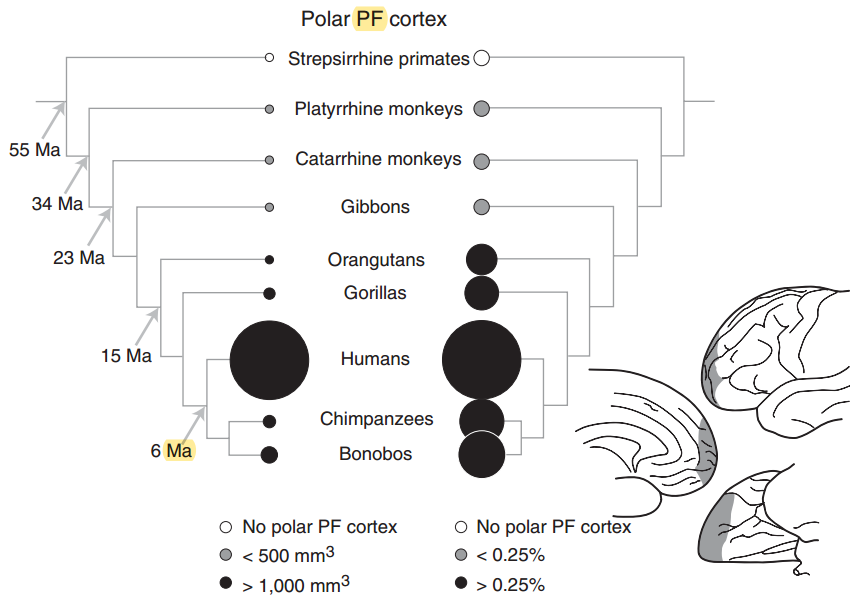
\includegraphics[width=0.5\linewidth]{image_pfc/Fig_9_1}
	\caption{人类额极皮层(区域10)的扩展。选定灵长类动物的分支图,左侧(箭头)的近似发散时间为数百万年(Ma)。
		每个圆圈的直径编码额极皮层的大小参数,由底部的比例给出,按每个分支图下方显示的灰度代码分类。插图显示了人类额极皮层的位置。左侧,内侧视图,嘴侧向右,背侧向上;顶部,右侧,侧视图,嘴侧向左,背侧向上;右下角,腹面观,嘴向左,侧面向上。从TsujimotoS、GenovesioA、WiseSP修改而来。认知科学趋势15:169–76,©2011,经爱思唯尔许可。\label{fig:fig_9_1}}
\end{figure}

\par
\begin{figure}[!htb]
	\centering
	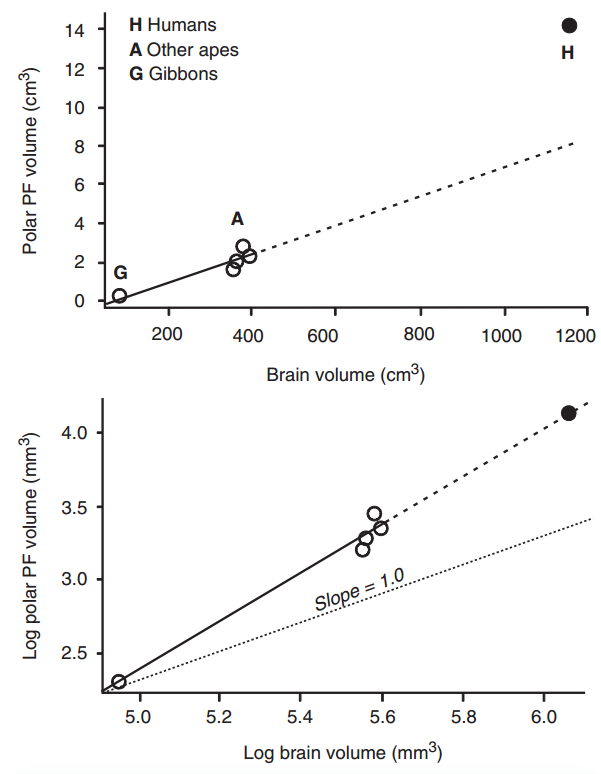
\includegraphics[width=0.5\linewidth]{image_pfc/Fig_9_2}
	\caption{在选定的灵长类动物群体中,额极皮层体积的回归作为脑体积的函数。实线:来自猿类数据的回归;虚线:外推到人类大脑的大小。顶部:线性刻度。底部:对数刻度,单位斜率由虚线表示。缩写:G,长臂猿;A,类人猿;哈,人类。修改自SemendeferiK、ArmstrongE、SchleicherA、ZillesK、VanHoesenGW。人类和类人猿的前额皮质:区域10的比较研究。美国体质人类学杂志114:224–41,©2001,JohnWileyandSons。\label{fig:fig_9_2}}
\end{figure}

\par

同一作者对第13区进行了类似的分析,发现与其他类人猿相比,人类没有这种扩张。
这些发现支持了额极皮层在人类进化过程中显着扩展的结论。
然而,霍洛威(2002)淡化了这些结果。
他指出,人脑额极皮层的大小仅比大脑与人脑一样大的猿类的预测大百分之六。
图\ref{fig:fig_9_2}显示了额极皮层大小与类人猿大脑大小的对数对数回归(桑德弗等人,2001年),它表明人类价值仅位于回归线上方。
\par


但是霍洛威(2002)假设如果人类额极皮层符合对数-对数回归线,或者接近符合,那么它具有相等的容量。
这种信念忽略了一个事实,即对数-对数回归线的斜率为1.6,大大超过了单位斜率(1.0)。
陡坡意味着较大的大脑比较小的大脑具有更大比例的额极皮层。
所以我们不能假设有类似的容量。
神经科学以外的一个例子解释了这一点(古尔德,1973)。
已灭绝的爱尔兰麋鹿有巨大的鹿角,但当将它们的长度与衡量体型(肩高)进行对比时,它们的长度接近回归线。
因为斜率超过了统一,所以它们的鹿角占身体的比例更大。
因此,它们的功能更有效,大概是在吸引配偶方面。
因此,结构符合回归线的事实并不意味着等效的功能能力。
\par



\textbf{总结}
\par

人脑不仅仅是猕猴和人类最后一个共同祖先的大脑的放大版。
大脑的某些部分比其他部分扩展得更多。
当考虑作为一个整体的新皮层的一部分时,颗粒状前额叶皮层在人类中比在猕猴中大~2.5。
\par


然而,大小只能告诉我们一点点,所以我们接下来考虑人类和其他大脑在微观结构和内部连接方面的差异。



\section{微观结构和内部连接}

在他们对额极皮层的研究中,桑德弗等人(2010)发现,与类人猿相比,人类第3层细胞体之间的这一区域存在大量神经纤维网。
换句话说,细胞体的间距更大。
与猿类相比,这种解剖学特征可能反映出人类有更多的树突、树突棘和末端。
这一特征指向颗粒前额叶皮层的综合功能的详细说明,一般而言,特别是额极皮层。
\par


埃尔斯顿(2001)测量了前额叶皮层第3层锥体细胞树突上的棘数。
他发现人类大脑中的这些细胞比猕猴大脑中的细胞多百分之七十。
由于连接终止于脊柱,这一发现意味着与猕猴相比,每个细胞都可以在人类前额叶皮层中整合更多信息。
\par


埃尔斯顿(2007)还绘制了各种灵长类动物(包括人类)的棘数与前额叶皮层大小的关系图。
他发现前额叶皮层越大,树突棘的数量就越多。
鉴于人类前额叶皮层的大尺寸,脊柱的数量与预期非常吻合。这似乎不是细胞大小增加的产物。
\par


内在联系在皮层下白质中运行,有两种类型。
申克等人(2005)区分位于白质核心的长联合纤维和连接前额叶皮层回旋内相邻区域的较短纤维。
他们比较了一些灵长类动物的这些值。
在人类中,包含长关联纤维的白质体积与人类大脑的预测一致。
然而,短纤维比人类预期的更广泛。
\par



\textbf{总结}
\par

在第\ref{chap:chap8}章中,我们回顾了证据表明,当一个人提升了针对上下文、目标和结果的各种处理层次时,刺的比例会增加。
我们认为,这种解剖学特征允许大脑在越来越抽象的层次上形成表征。
人类前额叶皮层可以将这种发展提升到一个新的水平。
此外,人类前额叶皮层似乎有大量短纤维将一个前额叶皮层连接到另一个。
因此,人类前额叶皮层可能特别适合整合信息。
在后面的部分中,我们提供证据表明前额叶皮层中的一些激活反映了整合来自不同认知领域的信息的能力。



\section{外部连接}

上一节考虑了连接数,但没有考虑远程连接的整体模式。
最近的研究利用了水沿着轴突在外部和内部扩散的事实。
这一特性催生了一种研究人脑连接的方法,称为扩散张量成像(DTI)。
施马曼等人(2007)使用这种方法的修改来绘制猴子的连接图,并发现类似于标准轴突纤维追踪方法的结果。
然而,DTI有严重的局限性。
这些方法永远不会像在猴子和其他动物身上使用的方法那样敏感,这些方法可以揭示微观水平上的联系,并且在足够重要的情况下,还可以揭示电子显微镜水平上的联系。
它们不能像猴子身上使用的方法那样揭示投射的确切起源和终止。
尽管如此,DTI数据提供了有关人类前额叶皮层连接的宝贵信息。
\par


克罗克森等人(2005)将前额叶皮层分为七个部分:背侧前额叶皮层、腹侧前额叶皮层、外侧眶额皮层、中央眶额皮层、内侧眶额皮层、前扣带回和扣带回。
他们使用哈伯德等人设计的方法测量了种子区域与另一个区域连接的可能性。
(2005),并发现人类前额叶皮层连接的一般模式与猴子相似。
例如,后顶叶皮层与背侧前额叶皮层相连,而下层颞皮层与腹侧前额叶皮层和眶额皮层相连。
在猴子和人类的大脑中,杏仁核都与眶额皮层和前扣带回皮层相连。
\par


同一组研究人员使用DTI将前扣带皮层分为九个区域(贝克曼内塔尔,2009)。
人脑的结果与猴子轴突纤维追踪研究的结果相似(卡迈克尔和普莱斯,1996)。
例如,在内侧前额叶皮层中,膝前和膝下区域与两个物种的眶额皮层、杏仁核、下丘脑和腹侧纹状体的联系最强。
\par


DTI还表明,丘脑内侧核(MD)和前额叶皮质之间的整体连接模式在人类和猴子中是相似的(克莱内塔尔,2010)。
MD的内侧部分与眶额皮层相连,尾侧MD与内侧前额叶皮层相连,包括前扣带皮层,外侧MD与背侧前额叶皮层相连。
\par


据我们所知,人类和猕猴前额叶皮层连接的整体模式似乎相似。
这种相似性大概反映了我们最后一个共同祖先的血统。
然而,现代猕猴和人类已经分别进化了20到3000万年,这意味着在任何一个谱系中都可能发展出特化。
在接下来的部分中,我们将指出人类大脑的三个可能的专业化:布罗卡区、额极皮层极的外侧部分和背侧扣带回皮层。



\section{布罗卡区}

布罗卡区,布罗德曼区44和45,位于腹侧运动前皮层(区域6)的前面。
从尾端到头端,腹侧前运动皮层是无颗粒的,44区是异常颗粒状的,45区是颗粒状的(石油醚,2005)。
在拓扑可比较的区域中,可以在猴子(图\ref{fig:fig_9_3})中发现相同的进展。
\par


克莱因等人(2007)使用DTI绘制了人脑中44和45区连接的整体模式。
他们得出结论,区域44和45以其连接区分,与细胞结构定义的区域44和45非常吻合(图\ref{fig:fig_9_3})。
DTI数据显示,在人脑中,44区与下顶叶皮层相连,45区与颞叶皮层相连(弗雷耶塔尔,2008)。
和克罗克森等人(2005)在猴子中使用DTI发现了相同的结果模式,彼得里德斯和潘迪亚使用标准示踪剂也是如此。
\par


里林等(2008)以这一发现为起点,比较了人类、黑猩猩和猴子的布罗卡区。
他们发现45区与中颞叶皮层的联系比44区更强。
里林等人比较了黑猩猩和人类,发现人类的中颞叶皮层与布罗卡区的联系比黑猩猩的更广泛。
最后,在人类中,这条通路在左半球比在右半球更大更广泛,而在黑猩猩中它是对称的。
随着儿童的成长,这些连接的强度在左半球增加,但在右半球却没有(帕斯等人,1999)。
\par


\begin{figure}[!htb]
	\centering
	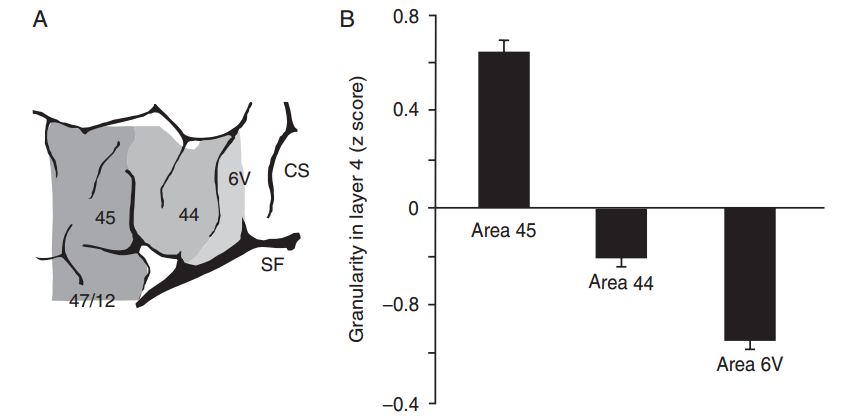
\includegraphics[width=0.5\linewidth]{image_pfc/Fig_9_3}
	\caption{(A)人脑中的布罗卡区。缩写:CS,中央沟;SF,外侧裂;6V,腹侧区域6。(B)猴子第4层的密度相对于相同三个额叶区域的平均值。经麦克米伦出版有限公司许可转载。布罗卡区猕猴同系物的口面部躯体运动反应。自然435:1235-8,©2005,自然出版集团。\label{fig:fig_9_3}}
\end{figure}

\par

布罗卡区在人类前额叶皮层左侧进化的想法当然不是什么新鲜事,但成像激活支持了这个想法。
人们可以记住发音(康拉德,1972)并且可以推理单词(高尔和多兰,2004)。当他们这样做时,成像激活往往发生在左半球。
但是当他们处理视觉空间信息时,激活往往发生在右半球(斯米泰塔尔,1996)。
尽管这里审查的比较证据还远非定论,但它似乎与在人类大脑中观察到的语言专业化大体一致。



\section{额极皮层}
对布罗卡区的研究表明,与人类和黑猩猩的最后共同祖先相比,人类的连通性发生了变化。
此外,文献包含暗示性证据表明人脑中的两个区域在猴子中缺乏同系物:
额极皮层的外侧部分,10区的一部分,以及背侧扣带回皮层,32区的一部分。
\par


塞门德费里等人(2001)表明额极皮层的外侧部分存在于类人猿和人类中,但不存在于猴子中。
如果被接受,这个想法将意味着它是在类人猿和人类的祖先中进化而来的。
然而,他们的结论完全取决于拓扑学和细胞构造证据。
鉴于后者取决于主观标准,需要更多的证据来接受这个想法,尽管它似乎有道理。
\par


纳尔逊等人(2010)发现了支持证据,其形式为下后顶叶皮层中心的激活与外侧额极皮层的激活之间存在相关性。
火星等(2011)比较了人类和猴子的静息状态相关性。
他们在中外侧前额叶皮层和额极皮层之间的边界上选择了一个感兴趣区域。
在人类中,该区域的静息激活与下顶叶皮层中央部分的激活相关,这与纳尔逊等人的发现一致。
但是火星等人没有在猴子中发现相应的相关性,这一发现与轴突运输研究中两个区域之间缺乏联系一致。
这些发现与外侧额极皮层(区域10)或与其相邻的区域在猴-猿分裂后进化的建议一致。
但是,需要进一步的证据证明这种可能性。
\par


如果额极皮层的外侧部分在人类和类人猿中进化,那么这个区域可以被视为位于处理层次结构的顶部。
萨默菲尔和德科奇林为外侧前额叶皮层提出了一个从尾端到头端的层次结构,它们与指定动作的上下文的复杂性有关。和德科奇林等人(1999)已经建议最延髓的部分,外侧区域10,在处理次要目标时牢有限数量的证据支持这样一种观点,即额极皮层极的外侧部分(区域10)出现在人类和猿脑中,但不存在于猴脑中。
它可能会在颗粒状前额叶皮层侧面的尾端到头端层次结构中创建一个新级别。



\section{背扣带旁皮层}

在有扣带旁沟的人脑中,32区背侧的扣带旁部分位于扣带沟和扣带旁沟之间(福格特,2009)。
在一些黑猩猩的大脑中也可以看到一个扣带旁沟,这个沟和扣带沟之间的皮层可能对应于人类的背侧扣带旁皮层。
我们需要更多的证据来证明。
\par


猴子也有一个称为32区(福格特,2009)的区域,但其细胞结构表明,它与人类的属前内侧前额叶皮层同源,而与背侧扣带旁皮层不同。
贸易部研究还提供了证据,证明背侧扣带旁皮层存在于人类而不存在于猴子。
在人类和猴子中,属前内侧前额叶皮层与杏仁核和下丘脑都有连接,但背侧扣带旁皮层缺乏这种连接(贝克曼,2009)。
然而,背扣带旁皮层确实与前额叶背侧皮层相连,科斯基和帕斯(2000)的元分析得出的结论是,背扣带旁皮层的激活倾向于与前额叶背侧皮层的激活相关。
这些数据提供了暗示性的证据,表明背扣带旁皮层是在猴猿分裂后进化的。



\textbf{总结}
\par

如果背侧扣带旁皮层只存在于人类和类人猿中,那么它可能像额极皮层一样,为前额叶皮层的尾侧至吻侧层级增加了一个额外的层次。对于极缘前额叶皮层,这个层次包括外侧前额叶皮层,但对于背侧扣带旁皮层,它包括内侧前额叶皮层。
其他人也提出了这种层次结构(阿莫迪奥和河口,2006;萨默菲尔德和科奇林,2009),我们稍后提出了支持这一观点的证据(见图\ref{fig:fig_9_7})。
在那里,我们提出,这些层次结构,无论是外侧和内侧前额叶皮层,都涉及到其较低水平处理的较高水平的信息的重新表征。
\par


我们并不是在暗示这里强调的三个领域是在猿类或人类进化过程中唯一出现的领域。
一些基于皮层髓鞘化程度的证据表明,47区(前额叶皮层腹侧的一个组成部分,称为47m区)的一小部分也可能出现在猿-人谱系中(格拉瑟,2011)。
来自同一研究的证据也支持这样一种观点,即颗粒状前额叶皮层,它有稀疏的髓鞘,在类人猿和人类的进化过程中急剧扩张。



\section{人类大脑的激活}
\par
如果我们承认猴子和人类的前额叶皮层是不同的,那么我们应该预料到它的功能也是不同的。
毕竟,现代猴子和人类已经分别进化了2000万到3000万年,他们走的是一条非常不同的道路。
然而,猴子和人类拥有共同的祖先,第\ref{chap:chap2}章解释了关于这些动物的一些事情。
在第\ref{chap:chap8}章中,我们提出了前额叶皮层的基本功能,因为灭绝的类人猿进化了它,而现代猴子继承了它。
因此,在本章的剩余部分,我们将探讨前额叶皮层的一些独特的人类功能是否可以被理解为我们共同祖先进化的基本功能的阐述。
\par


在接下来的章节中,我们将考虑影响认知心理学家关于人脑前额叶皮层功能观点的成像激活。
在许多情况下,我们建议如何根据我们在第\ref{chap:chap8}章中提出的建议来解释激活。
在某些情况下,当我们不能以直接的方式做到这一点时,我们会建议在人类进化过程中提出建议功能的方法。
\par


为了说明清楚,我们在一组表中列出了我们考虑的激活。
在每一节的开始,我们给出了该节中要考虑的激活表。
我们通过将激活与上下文、目标和结果层次结构(表9.1-9.5)联系起来组织了这些表,这些层次结构允许前额叶皮层将上下文映射到目标(表\ref{tab:9_6})。
最后三个表与基于事件(表\ref{tab:9_7})和抽象规则(表\ref{tab:9_8}和表\ref{tab:9_9})的目标生成有关。



\section{感觉处理}

我们提出,颗粒状前额叶皮层根据当前的上下文生成目标,并且它可以这样做,因为它位于上下文层次结构的顶部。
因此,表\ref{tab:9_1}列出了与上下文处理相关的激活。



\subsection{感觉决定}
\par

如果当前目标取决于上下文,则有必要识别该上下文。
在许多情况下,感官输入提供了明确而强烈的信号来传达当前环境,但这些输入通常不太清楚。


在这种情况下,主体必须做出感性决定。
如第\ref{chap:chap3}章所述,我们遵循夏尔(2001)将关于世界的感知决策与目标选择和行动选择区分开来。


希克伦(2006)展示了一组移动的点,被试必须决定这些点是向左移动还是向右移动。
实验者通过改变在同一方向上移动的点的比例来控制任务的难度,也就是连贯地。
为了识别可能与感知决定相关的激活,而不是选择或反应,希克伦等人引入了两个条件。
在一个实验中,受试者通过向左或向右扫视来报告他们的决定,而在另一个实验中,他们通过按左边或右边的按钮来报告他们的决定。
希克伦等人寻找这两种报告条件相同的激活。
\par


\begin{table}[htbp] 
	\newcommand{\tabincell}[2]{\begin{tabular}{@{}#1@{}}#2\end{tabular}} %换行指令
	\centering
	\caption{人类大脑的激活\label{tab:9_1}}
	\renewcommand\arraystretch{1.5}	%设置表格内行间距
	\begin{tabular}{lll}
		\toprule
		详细阐述 & 激活 & 与基本函数的关系\\
		\midrule
		 环境& 感官决策 & 识别环境  \\
		 & 感官意象 & 产生感官情境 \\
		&  感官意识 & 再现感官环境\\
				\bottomrule
	
	\end{tabular}%
\end{table}%


希克伦等人在背侧前额叶皮层、额极皮层以及后顶叶皮层发现了满足这一要求的激活。
在之前的一项研究中(希克伦,2004),同一作者发现,当受试者必须判断退化的图像是房子还是脸时,背侧前额叶皮层会被激活。
\par


希克伦等人(2006)认为他们的结果与猴子的结果有很大不同。
他们声称,人类前额叶皮层的激活反映了决策或感知,而猴子前额叶皮层的活动反映了计划好的行动或视觉运动的关联。
他们假设,当猴子通过扫视来报告移动点的方向时,前额叶细胞的活动会编码相应的扫视(金和沙德伦,1999)。
\par


尽管他们得出了这样的结论,但人类和猴子的实验结果是完全一致的。
鋆和沙德伦(2007)在训练猴子对红色或绿色目标进行扫射后,通过对额叶视区进行微刺激来报告连贯点运动的方向。
猴子事先不知道每个目标会出现在哪一边,因此无法准备扫视。
刺激影响目标的选择,而不是扫视的方向。
因此,尾侧前额叶皮层的活动反映的是目标,而不是猴子为实现目标而采取的行动。
希克伦所报告的激活可以用同样的方式来解释:它们可以反映目标(比如左边),而不管受试者是按下左边的按钮还是向左边扫视。
\par


希克伦等人的结论的另一个问题是把体素当作细胞来处理。
第\ref{chap:chap1}章解释了做出这种假设的危险。
考虑到每个体素包含数千个细胞,并且血液信号反映的是突触而不是细胞活动,体素中的一些细胞更有可能编码感知决策,而其他细胞编码基于该决策产生的目标。
在一项对猴子的研究中,列别捷夫(2001)发现猴子的前额叶皮层中的细胞反映了它们报告的幻觉运动方向,无论猴子用来报告的扫视方向如何,这些细胞都表现出类似的活动。
但表现出这种特性的细胞亚群与直接向可见目标编码扫视的细胞混合在一起。
成像实验无法对这些混杂的细胞群和驱动活动的突触输入进行分类。
\par


列别捷夫等人得出结论,前额叶皮层能够将与当前情境相对应的感知信息与在该情境基础上生成的目标选择结合起来。
我们认为没有理由对人类受试者的成像激活有任何不同的解释。
因此,希克伦等人的研究结果与我们在第\ref{chap:chap8}章中提出的建议一致。
我们认为,前额叶皮层位于上下文层次结构的顶端,这意味着它可以识别当前上下文并生成适当的目标。
人类可以在不产生任何目标的情况下思考这些情境,我们物种的大部分精神生活都致力于这样做。
然而,这种能力并不表明人类和猴子的前额叶皮层有任何根本区别。



\subsection{感官意象}
\par

人们不仅可以对面孔和房子等刺激做出决定,他们还可以想象这些刺激。
当他们这样做时,激活发生在中外侧前额叶皮层(伊沙伊,2000)和腹侧前额叶皮层(伊沙伊,2002)。
然而,当受试者只是看到脸和房子时,很少会出现前额叶激活。
哈萨比斯等人(2007a)特别比较了观察到的物体和想象物体的记忆。
腹侧前额叶皮层在想象熟悉和新物体时表现出增加的激活。
\par


想象面孔和房子也会激活颞叶。
就像受试者看到脸或房子时,激活的位置不同一样,当受试者想象它们时,激活的位置也不同(伊沙伊,2000)。
为了测试这种激活是否依赖于来自前额叶皮层的自上而下的影响,或者依赖于后顶叶皮层,梅凯利等人(2004)使用了一种统计方法,允许他们分析一个区域对另一个区域的影响。他们研究了在对面孔、房屋和椅子进行想象时大脑皮层的相互作用。
颗粒状前额叶皮层与颞叶的不同部分相互作用取决于图像的内容,但后顶叶皮层的激活没有。
这一发现与前额叶皮层产生假想情境的观点一致。
\par


生成图像从两个方面反映了前额叶皮层的基本功能。
\par


首先,图像的表示类似于当前上下文,特别是存储在内存中的上下文。
第二,正如第\ref{chap:chap8}章所解释的那样,粒状前额叶皮层开始参与注意力要求,而不是自动控制行为,而想象需要注意力。
\par


布鲁耶和斯克兰奇(1998)使用的双任务范式阐明了这一点。他们要求受试者想象一个地方有字母,然后问他们同一个地方是否出现了探针(科斯林,1995)。
当受试者必须同时生成随机数,从而迫使注意力控制时,他们在生成图像时犯了许多错误。
然而,一旦他们生成了虚构的字母,受试者就可以在不受随机数任务干扰的情况下将它们保存在记忆中。
因此,生成图像需要注意控制和前额叶皮层的参与。
\par


在后面的小节中,我们将讨论其他需要主体生成表示的任务。
例如,当受试者用名词生成动词时,腹侧前额叶皮层就会被激活。
当出现“蛋糕”时,受试者可能会产生“吃”或“切”。
然而, 当实验者重复呈现相同的名词列表,并且被试对他们做出刻板反应时,没有明显的激活发生(赖歇尔,1994)。
这些结果支持了上下文表征的注意生成依赖于前额叶皮层的说法,从而解释了在此类任务中观察到的激活。



\subsection{感官意识}

鉴于前额叶皮层位于情境层次结构的顶端,有人认为它可能对感知感官刺激至关重要(克里克和科赫,1998)。
许多影像学研究比较了有意识和没有意识的情况(里斯,2002)。
\par


其中一个例子涉及到变化盲目性。
贝克(2001)集中呈现字母,并要求受试者执行字母检测任务。
图片出现在周边,在某些情况下,它们从一个显示到另一个显示。
实验者改变了字母任务的难度,因此在一些试验中,受试者注意到了外围的变化,而在另一些试验中,他们没有注意到。
意识与后外侧前额叶皮层和尾侧前额叶皮层以及后顶叶皮层的激活相关。
\par


反向屏蔽还可以防止感知。
在这个过程中,一个刺激迅速地跟随另一个刺激。
两个刺激之间的间隔很短,30毫秒左右,第二个刺激可以阻断第一个刺激的意识。
刘和帕辛厄姆(2006)使用了这种技术,他们调整了两种刺激的时间,以使受试者在两种情况下察觉到或没有察觉到第一种刺激的试验百分比相等。
\par


受试者必须说出目标刺激是正方形还是菱形,这两种条件是相匹配的,以确定受试者能够做到这一点的准确性。
\par


然而,在试验中受试者说他们“看到”刺激的比例上,不同的条件有所不同。
在一些正确的测试中,受试者觉得他们是在猜,尽管是对的。
当受试者判断他们已经“看到”刺激时,中外侧前额叶皮层的激活程度比他们只是“猜测”他们已经看到刺激时要高。
\par


如果前额叶皮层对感觉意识是必要的,前额叶皮层损伤应该会干扰意识。
因此,在随后的一项研究中,鲁尼斯等人(2010)在受试者执行后向掩蔽任务之前,将重复经颅磁脑刺激(rTMS)应用于双侧前额叶皮层。
他们以θ频率刺激以抑制受影响区域的活动;然后他们对受试者进行测试(黄,2005)。
暂时的失活对受试者判断目标刺激的准确性没有影响。然而,它确实影响了受试者报告他们“看到”刺激的试验比例。
\par


德尔库尔等人(2009)也使用后向掩蔽技术,测试额叶皮层病变患者识别手指的能力。
作者通过在患者的目标刺激后延迟掩蔽刺激的时间比对照组的时间更长来匹配患者和对照组的表现。
正如刚刚提到的研究所预期的那样,前额叶皮层病变的患者表示,他们比健康的受试者更少“看到”手指,特别是当病变包括左额极皮层时。
因此,前额叶皮层的激活似乎与一种反思意识有关,这是指一个人对自己看到某事的信心。
\par


\textbf{总结}
\par

第\ref{chap:chap8}章表明,前额叶皮层位于上下文层次结构的顶端。
它还认为,当一个人在这个层次结构中上升时,较高的层次重新表示较低层次处理的信息,而且他们通常以更抽象的形式这样做。
由于前额叶皮层位于上下文层次结构的顶端,它可以重新表示一个人的感知判断,并根据这些判断做出决定。
向上下文层次结构中添加一个新级别可能是这个函数的基础,稍后我们将回到这个主题。



\section{目标的产生}
\par

第\ref{chap:chap8}章强调具体目标,如物体或位置。
但是人类会产生各种各样的目标。
有时一个单词可以是一个目标,例如当一个人在记忆中搜索一个单词时。
所以表\ref{tab:9_2}扩展了我们到目前为止所使用的目标的概念。



\subsection{动词的一代}
\par
在早期的一篇论文中,彼得森等人(1988)使用正电子发射断层扫描(PET)来记录人们生成与特定名词相对应的动词时的激活情况。
\par

生成哪个动词是由个人决定的。所以,对于“蛋糕”这个名词,他们可能会说“吃”、“切”或“做”。
在对比条件下,被试只是简单地重复这个名词。
\par

当彼得森等人比较这两种情况时,当受试者产生动词时,前额叶皮层发生了更多的激活。
随后的研究表明,激活的峰值出现在腹侧前额叶皮层(巴克纳,1995)。
如前所述,当受试者重复看到相同的名词列表时,他们倾向于对特定的名词做出相同的动词反应(赖歇尔,1994)。
当他们的选择以这种方式成为刻板印象时,前额叶皮层的激活不再超过对照条件。
\par


这些结果表明,前额叶皮层激活反映了目标项目的注意生成,在这种情况下,一个动词适合于一个给定的名词。
然而,彼得森等人的发现还有另一个重要的含义。
在动词生成中,名词提供了当前上下文,因此激活也可以反映出适合该上下文的目标的生成。
\par


\begin{table}[htbp] 
	\newcommand{\tabincell}[2]{\begin{tabular}{@{}#1@{}}#2\end{tabular}} %换行指令
	\centering
	\caption{人类大脑的激活\label{tab:9_2}}
	\renewcommand\arraystretch{1.5}	%设置表格内行间距
	\begin{tabular}{lll}
		\toprule
		详细阐述 & 激活 & 与基本函数的关系\\
		\midrule
		目标 & 动词的一代 & 根据上下文生成目标项  \\
		& 想象动作 & 生成适合上下文的目标 \\
		&  计划 & 生成一系列目标 \\
		\bottomrule
		
	\end{tabular}%
\end{table}%


这些结果表明,前额叶皮层激活反映了目标项目的注意生成,在这种情况下,一个动词适合于一个给定的名词。
然而,彼得森等人的发现还有另一个重要的含义。
在动词生成中,名词提供了当前上下文,因此激活也可以反映出适合该上下文的目标的生成。
见过“他寄这封信时没有附页…”,这让大多数人产生了“邮票 ”。
对比的条件几乎没有限制。
当受试者看到像“警察从未见过如此……的人”这样的句子时,他们可以生成许多单词,如“醉酒”、“邪恶”等。
纳撒尼尔-詹姆斯发现,在无约束条件下,与有约束条件下相比,中外侧前额叶皮层被激活。
\par


这些激活遵循第\ref{chap:chap8}章提出的功能,因为这些任务涉及适当于上下文的目标的注意生成。



\subsection{想象动作}

在前面的部分中,我们回顾了与视觉图像的“内部”生成相关的激活。但人们也可以想象行动。
例如,热拉丁(2000)要求受试者做简单的手指动作或更复杂的手指动作。
\par


在这两种情况下,前额叶皮层都没有发生任何激活。
然而,当受试者必须想象进行相同的动作时,颗粒状前额叶皮层显示出明显的激活埃尔松等人(2003)后来证实了这一结果。
\par


运动想象任务通常也会导致前额叶皮层外的激活。
热拉丁等人和热拉丁等人的任务导致了吻侧前运动皮层和后顶叶皮层的激活。
这样的结果并不令人惊讶,因为运动想象很可能涉及到运动的准备(让纳罗德,2006),并且当受试者准备运动时,运动前皮层和后顶叶皮层都被激活(托尼,2002)。
\par


罗(2002)并没有要求受试者想象动作,而是指导他们在不想象的情况下思考即将到来的动作。
正如前面所解释的,在视觉图像的研究中,关键问题涉及到三个区域之间的层次结构,其中始终包括前额叶皮层和后顶叶皮层。
在视觉图像方面,第三个区域是颞下皮层;在运动意象方面,是运动前皮层。
与视觉图像的结果一样,罗等人的分析表明,对第三区域的关键影响来自前额叶皮层,而不是后顶叶皮层。
\par


这一结果的关键因素涉及注意力。
当运动准备对注意力产生要求时,前额叶皮层就会被激活。
罗等人发现,只有当受试者必须关注下一个目标时,前额叶皮层才会被激活。
当他们在执行一系列动作的同时进行视觉搜索任务,从而转移注意力时,前额叶皮层对运动前皮层的影响下降。
\par


就像感官意象一样,想象一个动作涉及到对表象的注意生成。
在感官意象的情况下,这种表征与上下文有关;在运动意象的例子中,它与动作有关。
我们在第\ref{chap:chap8}章中认为,与后顶叶皮层不同,前额叶皮层可以产生这些表征,因为它位于上下文和目标层次结构的顶部。
\par



\subsection{规划}

人们还可以想象一系列的目标。
在实验室里,心理学家通过需要一系列步骤才能达成解决方案的任务来评估这种计划。
例如, 在“河内塔”任务中,受试者必须重新排列颜色的环,以便在最少的步骤内实现给定的目标排列。
一个简化的版本,叫做伦敦塔任务,使用三根棍子和三个彩色球(沙利斯,1982)。问题可能需要两步、三步、四步或五步。
\par


道格等人(1999)发现,当受试者执行伦敦塔任务时,中外侧前额叶皮层被激活,而当解决方案需要更多步骤时,额极皮层被激活。
无论受试者只是计划步骤,还是两者都计划并执行它们,都会发生类似的激活。
\par


虽然这些区域在规划过程中被激活,但这一发现并没有显示这些激活反映了什么过程。
例如,我们知道更困难的问题涉及反直觉的运动,例如圆盘或球远离其最终目的地的运动(戈尔和格拉夫曼,1995)。
戈尔和格拉夫曼(1995)的研究表明,额叶病变患者在需要这种动作时往往会出错。
\par


然而,还有另一个问题,那就是激活可能与解决问题有关,而不是计划本身。
有些任务,比如河内塔,既需要解决问题又需要规划。
在日常生活中,人们计划一系列不需要解决太多问题的目标,比如购物旅行。
因此,沙利斯和伯吉斯(1991)让三名前额部有大面积病变的患者在一家购物中心做了一系列的差事。
这些差事包括,例如,买一条面包,实验人员指示患者不要去同一家商店两次。
\par


不幸的是,这些患者中只有1例出现病变,且该大病变涉及额极和眶吻侧表面(沙利斯和库珀,2011)。
因此,特内尔等人(2007)在大量患者中重复了这项研究,并根据结构成像描述了他们的病变。
表现不佳的患者有双侧病变,不仅包括额叶腹侧和内侧的大部分,而且还包括额极皮层。
\par


当然,不能在实验对象执行任务时对他们进行成像实验。但如果只是简单地要求受试者描述购买食品杂货所需的一系列步骤,就可以做到这一点。
古德博特和多永(1995)要求受试者生成这样的脚本,他们发现额叶病变患者生成的步骤更少,而序列错误更多。
\par


\textbf{总结}

就像人们可以产生视觉图像一样,他们也可以想象行动。这使他们能够计划,并做到遥远的未来。
当人们在伦敦塔的任务上计划移动时,对于难度越大的问题,激活延伸到额极皮层的横向部分(多永,1999),而难度越大的问题涉及反直觉的移动。
在这些问题上,受试者必须牢记最终目标,同时计划偏离该目标的附属行动。
如前所述,科奇林等人(1999)表明,这种情况特别涉及额极皮层。
这些激活反映了目标层次结构的细化,可能是通过添加一个新的级别。我们稍后再讨论这种可能性。



\section{任务说明}
\par

当人们执行实验室任务或外出办事时,实验者首先告诉他们该做什么。
这意味着当受试者执行任务时,他们需要记住他们应该做什么。
表\ref{tab:9_3}列出了涉及在内存中维护任务的两种情况下的激活。
在第一种情况下,受试者必须在短期记忆中保持任务。
在第二种情况下,受试者执行两项任务,他们需要在执行另一项任务时将其中一项保持在短期或长期记忆中。



\subsection{在内存中维护当前任务规则}
\par

正如第\ref{chap:chap7}章所提到的,沃利斯等人(2001)通过训练猴子将低音调作为应用匹配规则的指令,将高音调作为应用不匹配规则的指令,来教导猴子在任何给定的试验中是否适用匹配规则或不匹配规则。
在一个相关的成像实验中,邦吉等人(2003)教人类受试者一个无意义的声音“pohu”表示匹配,另一个无意义的声音“siba”表示不匹配。
在每次试验中,其中一个指令在延迟期之前出现,选择项在延迟期之后出现。
在延迟期间,前部腹侧皮层被激活。
\par


酒井和帕辛厄姆(2003,2006)在两个实验中使用英语单词指导受试者应该执行什么任务,而不是向受试者呈现无意义的单词。
在第一个实验中,受试者看到一系列的四个位置和字母。
\par


在看到这些刺激之前,受试者已经收到了一个指令,要么记住字母或它们的位置,要么按照它们出现的顺序或相反的顺序去做(酒井和帕辛厄姆,2003)。
在第二个实验中,受试者在看到一个名词后,被要求报告对这个词的语义判断(抽象还是具体)或语音判断(两个音节还是一个或三个音节)。


\begin{table}[htbp] 
	\newcommand{\tabincell}[2]{\begin{tabular}{@{}#1@{}}#2\end{tabular}} %换行指令
	\centering
	\caption{人类大脑的激活\label{tab:9_3}}
	\renewcommand\arraystretch{1.5}	%设置表格内行间距
	\begin{tabular}{lll}
		\toprule
		详细阐述 & 激活 & 与基本函数的关系\\
		\midrule
		目标 & 在内存中维护任务规则 & 任务规则的前瞻记忆  \\
		& 在内存中维护未来的任务 & 未来任务的前瞻记忆 \\
		\bottomrule
		
	\end{tabular}%
\end{table}%
\par


在这两项研究中,作者都发现在延迟期间腹侧前部皮层的吻侧部分被激活。
在最初的论文中,这种活动被描述为发生在额极,但更准确的说法是,这种活动发生在靠近极地前部皮层边界的某个地方。
作者将这种激活解释为任务集的反映。
从这个意义上说,任务集指的是在任何给定时间指导行为的规则。
在第一项研究中,当受试者需要记住顺序相反的位置时,任务集的激活与尾侧前部皮层的激活关系更好;当受试者需要记住顺序相反的字母时,与布洛卡区(在左腹侧前部皮层的另一部分)的激活关系更好。
在第二项研究中,任务集激活与腹侧运动前皮层激活的相关性更好。
当被试需要进行语音判断时,被试需要读出单词,而当被试需要进行语义判断时,左腹侧前部皮层的尾侧部分被激活的效果更好(图\ref{fig:fig_9_4})。


\begin{figure}[!htb]
	\centering
	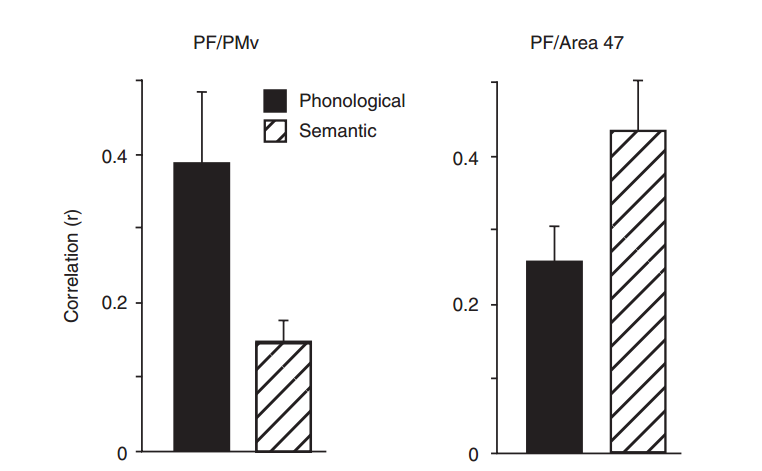
\includegraphics[width=0.5\linewidth]{image_pfc/Fig_9_4}
	\caption{在两个任务中,一个是语音任务(黑条),一个是语义任务(黑线条),吻侧前部皮层与一个更尾端、任务特定区域的激活关系。前额叶/PMv:吻侧前额叶皮层和腹侧运动前皮层延迟期激活的相关性。前额叶/ 47区:延迟期激活在吻侧前额叶皮层和47区下部的相关性。误差条:SEM。摘自Sakai K, Passingham RE。在随后的认知表现中,前额叶集活动预测规则特异性神经处理。神经科学杂志26:12 - 18,©2006,神经科学学会,已获许可。\label{fig:fig_9_4}}
\end{figure}
\par


可以认为,延迟相关的激活反映了对任务指令的记忆,而不是对执行特定任务的准备。
但是海恩斯等人的一项研究(2007)排除了这种解释。
他们的任务不涉及任何口头指示。
相反,在每次试验开始时,受试者决定执行什么操作,具体来说是加还是减数字。
然后在数字出现之前出现可变延迟。
作者使用一种区分不同试验类型激活模式的方法分析了不同前额叶皮层的延迟期激活。
尽管缺乏口头指令,模式分析器可以检测受试者是否会加减,正确率为百分之六十到七十。
\par


如果任务集激活反映了内存中任务的维护,那么对具有这种激活的区域的损害应该导致错误并改变特定于任务的区域的激活。
因此,罗等人(2007)研究了4名患有较大额外侧病变的患者。
患者和对照组受试者看到出现在四个位置中的任何一个位置的一系列字母,他们必须记住位置或字母(图\ref{fig:fig_9_5})。
当指令从一个试验转换到下一个试验(轮班试验)时,前额叶皮层病变患者比健康人犯更多的错误。
另一方面,如果指令一次又一次地重复,他们犯的错误就比对照组少(停留试验)。
罗等人对这一结果的解释是,患者未能将当前任务保留在记忆中,而默认情况下重复了与前一次试验相同的任务。
\par


\begin{figure}[!htb]
	\centering
	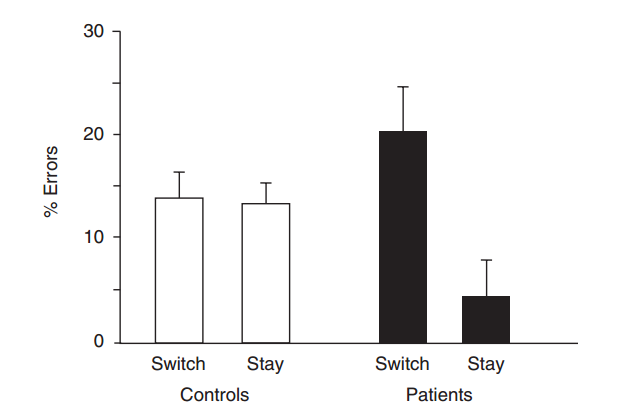
\includegraphics[width=0.5\linewidth]{image_pfc/Fig_9_5}
	\caption{罗等对患者(黑条)和对照组(白条)的记忆和注意选择任务的行为结果。纵坐标:记忆位置或字母错误的百分比。在停留试验中,任务与前一次试验相同;在切换试验中,任务与前一次试验相反。误差条:SEM。摘自罗杰比,酒井,隆德,拉姆索伊,克里斯滕森,巴雷,保尔森, 帕辛厄姆。前额叶皮层是建立认知集的必要条件吗?神经科学杂志27:13303-10,©2007,神经科学学会,已获许可。\label{fig:fig_9_5}}
\end{figure}

\par


罗等人还分析了尾侧前额叶皮层和后顶叶皮层延迟期激活之间的相关性,以及尾侧额下回(布罗卡区)和颞叶皮层之间的相关性。
他们发现患者的相关性低于对照组(图\ref{fig:fig_9_6})。
停留试验和轮班试验都是如此。
结果表明,这种损伤破坏了尾侧前额叶皮层和与之相连的特定任务区域之间的激活协方差。
\par


\begin{figure}[!htb]
	\centering
	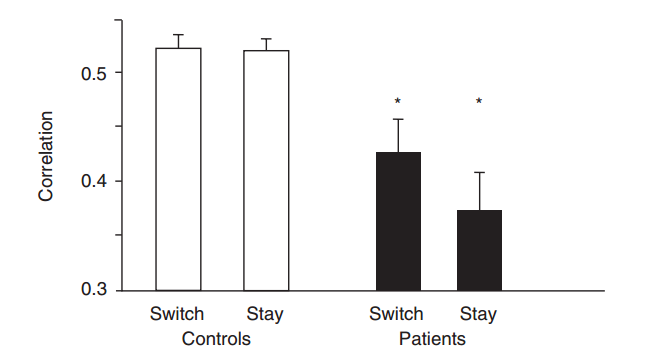
\includegraphics[width=0.5\linewidth]{image_pfc/Fig_9_6}
	\caption{罗等人使用的任务成像结果,患者(黑条)和对照组(白条)。尾侧前部皮层延迟期激活与顶叶和颞叶任务相关区域之间的相关性。留庭审判和轮班审判分别进行。摘自罗杰比,酒井,隆德,拉姆索伊,克里斯滕森,巴雷,保尔森,帕辛厄姆。前额叶皮层是建立认知集的必要条件吗?神经科学杂志27:13303-10,©2007神经科学学会,已获许可。\label{fig:fig_9_6}}
\end{figure}

\par

这些发现与前皮层的基本功能有关,因为它们表明前皮层参与维持记忆中当前任务规则。
回想一下,第\ref{chap:chap8}章中的建议是指颗粒状的前额叶皮层提供了一种学习和应用抽象规则的机制。



\subsection{在内存中维护未来的任务}
\par

在刚才提到的研究中,受试者在每次试验中执行一项任务。
但受试者在每次试验中也可以执行两项任务,在这种情况下,他们需要在执行另一项任务的同时保持一项任务的记忆。
“前景”一词已经在这种有限的意义上使用(伯吉斯,2000)。
我们把这种用法放在引号里是因为我们以不同的方式使用同一个术语(参见术语表)。
\par


在我们之前提到的一项研究中,科奇林等人(1999)要求受试者匹配一系列大写字母,按右键表示匹配,按左键表示不匹配。
在分支条件下,受试者需要判断大写字母是否匹配,同时执行次要任务。
第二项任务要求他们在大小写发生变化时记下小写字母“t”。
在比较条件下,受试者在这两项任务之间交替进行。
在分支条件下,额极皮层比交替条件下更活跃,可能是因为它使受试者能够在将注意力转移到更直接的次要任务时暂停主要任务的执行。
\par


如果极区前部皮层(10区)在同时保持两个任务的记忆中起着特殊的作用,那么人们就会认为该区域受损的患者在这方面表现不佳。
在两项研究中,伯吉斯及其同事给了患者一系列简单的任务,并要求他们完成所有任务(伯吉斯,2000,2007)。
与健康人相比,患者尝试的任务更少,在任务之间切换的频率也更低。
作者的结论是,患者在尝试时并没有将所有的任务都保存在前瞻记忆中。
因此,人类的额极皮层似乎支持多任务处理行为。
\par


然而,侧额极皮层不仅仅是在记忆中保存多个任务。
它还可以在内存中保存多个潜在目标。
布尔曼等人(2009)在受试者从两个类似物体的目标中做出选择时对其进行扫描。
他们发现,侧额极皮层的激活与备选选择的相对优势相关,即未选择的潜在目标。
在一项涉及多个备选方案的后续研究中,侧额极皮层的激活反映了这些未选方案中最佳方案的奖励价值(布尔曼,2011)。
随后,我们讨论了侧额极皮层代表潜在选择的可能性,并评估了每种选择的可能结果。
这种认知操作相当于在想象中进行的试错行为,我们认为这种能力对人类的认知做出了至关重要的贡献。
\par



\textbf{总结}
\par
在我们的建议中,我们认为当猴子不能立即行动时,前脑皮层可以对目标进行前瞻性编码,直到行动的时间到来。
然而,区分目标的前瞻编码和从长期记忆中提取它们是很重要的。
如果患者有较大的吻侧前部前部病变,包括极侧前部前部皮层,如果被要求,可以重复说明;但他们往往不能将其付诸实践,例如,在执行一系列三个简单任务时(伯吉斯,2000)。
他们之所以能背诵指令,可能是因为当被问及这些指令时,病人能从长期记忆中检索到适当的表征。
尽管这种能力完好无损,但同样的患者在执行一系列任务时必须在记忆中保持这些表征的能力受损。
我们认为,以这种方式维持目标表征的失败导致了邓肯等人(2008)所说的目标忽视。



\section{监控的意图}
\par
涉及目标层次结构的最后一组激活涉及对意图的监视。
表\ref{tab:9_4}给出了这里考虑的两个激活。
\par


\subsection{监控自己的意图}
\par
我们在第\ref{chap:chap8}章中提出,与自动控制相比,前叶皮层会专注地产生目标,我们在本章中提供的数据显示,当人类受试者专注于他们正在做的事情时,前叶皮层会激活(罗等人,2002)。
受试者进行一系列的手指运动,而实验者只是告诉受试者思考他们的动作。
\par


简单地告诉受试者注意他们的行为是一种不优雅的操纵注意力的方式。
因此,在后来的研究中,刘(2004)使用了利贝特及其同事(1983)引入的任务。
在这项任务中,受试者被指示随时移动手指。
为了使被试能够确定他们的意图,一个点在一个钟面周围移动,被试必须注意并记住当他们第一次意识到他们的行为意图时,这个点的位置。
这个位置对应一个时间,被试通常报告他们的目标意识在运动开始前200毫秒左右发生。
\par


刘等人(2004)在一个成像实验中使用了这个任务。
在一种情况下,受试者必须报告他们何时意识到自己要移动手指,而在比较条件下,他们只需报告他们实际移动手指的时间。
与后一种情况相比,关于意图的报告与前SMA、后顶叶皮层和中外侧前额叶皮层(46区)的激活有关。
受试者报告意识的时间越早,激活程度越高(刘,2006)。
激活位于前SMA和SMA之间的边界,如图\ref{fig:fig_9_7}(第2点)所示。
\par


\begin{table}[htbp] 
	\newcommand{\tabincell}[2]{\begin{tabular}{@{}#1@{}}#2\end{tabular}} %换行指令
	\centering
	\caption{人类大脑的激活\label{tab:9_4}}
	\renewcommand\arraystretch{1.5}	%设置表格内行间距
	\begin{tabular}{lll}
		\toprule
		详细阐述 & 激活 & 与基本函数的关系\\
		\midrule
		目标 & 监控自己的意图 & 注意行动  \\
		& 监视他人的意图 & 用手势来预测他人的行为 \\
		\bottomrule
		
	\end{tabular}%
\end{table}%


\begin{figure}[!htb]
	\centering
	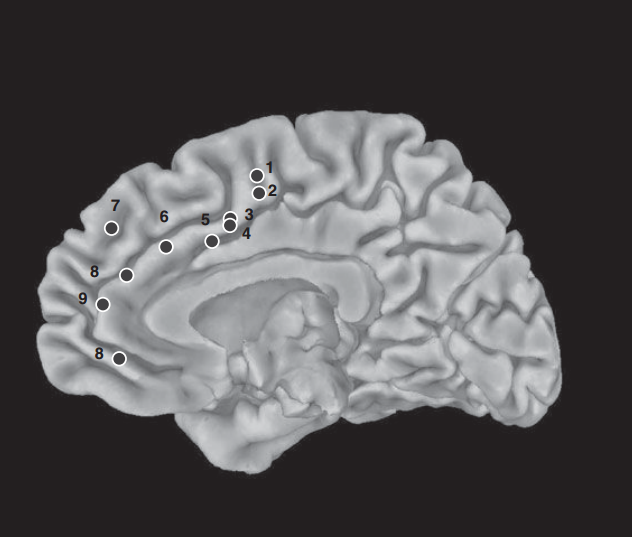
\includegraphics[width=0.5\linewidth]{image_pfc/Fig_9_7}
	\caption{图9.7反映几个认知过程的内侧激活的峰值体素:1,对动作的注意;2、注意意图;3、注意饥饿;4、注意情感;5、注意心率;6、关于自身特质词的反思;对自己表现的反思;8(两座高峰),回忆自己生活中的片段;第九,对他人精神状态的反思。内侧观,吻侧在左边。\label{fig:fig_9_7}}
\end{figure}

\par


在随后的实验中,刘等人(2006)发现,当受试者报告他们实际移动手指时,尾状扣带运动区会被激活图\ref{fig:fig_9_7}

第1点)。
刘等人分析了人们报告意图时三个激活位点之间的协方差,发现前额叶皮层对前SMA有显著影响,但后顶叶皮层对前SMA没有影响。
\par


在这些实验中,受试者只需报告他们第一次意识到某种特定精神状态的时间。
然而,人类受试者可以对自己的精神状态做出其他判断。
例如,在居斯纳尔(2001)的一项实验中,受试者观看一系列图片,并根据图片给他们的感觉是愉快还是不愉快,按下两个键中的一个。
居斯纳尔等人称之为内省条件。
在对比条件下,受试者根据场景是室内还是室外按下按键。
在内省条件下,背扣带皮层和背内侧前额叶皮层(9区)的激活更多,当受试者判断图片是否使他们感到兴奋或警觉时,也有类似的结果(戈德堡,2006)。
\par


在赫维格等人(2010)的一项实验中,受试者要么思考他们的目标,要么思考他们的情绪。
目标激活发生在背扣带皮层,情绪激活发生在更后方的前扣带皮层。
图\ref{fig:fig_9_7}反映几个认知过程的内侧激活的峰值体素:1,注意动作;2、注意意图;3、注意饥饿;4、注意情感;5、注意心率;6、关于自身特质词的反思;对自己表现的反思;8(两座高峰),回忆自己生活中的片段;第九,对他人精神状态的反思。
内侧观,吻侧在左边。当受试者对自己的精神状态做出判断时,皮层(9区)变得更加活跃,但当受试者对刺激物做出判断时,激活程度降低(居斯纳尔,2001;赫维格,2010)。



\subsection{监视他人的意图}
\par
弗里思(2007)认为,人们之所以有能力表达他人的意图,是因为他们能够表达自己的意图。
在大多数受试者判断他人精神状态的研究中,激活发生在背旁扣带皮层或内侧前部皮层的邻近部分(阿莫迪奥和河口,2006)。
图\ref{fig:fig_9_7}中的第9点显示了来自荟萃分析的峰值激活(吉尔伯特,2007)。
\par


成像激活也揭示了对他人和对自己的判断之间的关系。
当受试者决定一个特定的特征是否适用于自己时,激活发生在背扣带皮层(图\ref{fig:fig_9_7}第6点)。
当他们决定这些特征词是否适用于其他人时,激活的高峰出现在几乎相同的地方(奥克斯纳,2005)。
\par


在人类社会中,读懂别人的意图有很多好处。
其中一个不太明显的是模仿。
人们可以仅仅通过模仿观察到的行为来模仿,但是当一个人试图通过模仿别人的行为来达到同样的目标时,这种行为就变得更加重要了。
奘等人(2011)在观察某人制作燧石工具时,对新手和专家进行了扫描。
他们的实验涉及两种类型的工具:一种是奥尔德瓦式砍刀,通过简单地将燧石片从岩心上敲下来制成;另一种是阿舍利式手斧,通过在岩心边缘进行一系列复杂的击打,以产生连续的刀片。
\par


在新手和专家中,当观察复杂的手斧和简单的砍刀的制造时,腹侧前部皮层的激活程度都更高。
然而,只有在专家中,激活也发生在内侧前部皮层。
奘等人认为,这反映了一个事实,即专家比新手更能理解工具制造商的意图。
\par


\textbf{总结}
\par

当人们关注自己的行为时,前SMA会被激活,而当人们监控自己的意图时,背扣带皮层、背内侧前部皮层(9区)和内侧前部皮层的其他部分会更明显地被激活。
监控自己意图的能力意味着人们也可以监控自己的其他心理状态,这种能力使他们能够读懂别人的心理状态。
阿莫迪奥和河口(2006)指出,对他人心理状态进行反思的激活通常位于内侧前额叶皮层的尾部(图\ref{fig:fig_9_7}中的第9点),而监视自己意图和运动的激活则位于更尾部(图\ref{fig:fig_9_7}中的第2点和第1点)。
我们之前提出过内侧前部皮层的吻侧部分,背扣带皮层,可能是在人猿谱系中进化而来的。
\par


在本节讨论的激活的背景下,这个区域可能详细说明了猿和人类继承的目标层次,从而提供了一种新的能力。
我们将在本章的结束语中再次讨论这个问题。



\section{监测结果}
\par
现在我们转向涉及结果监视的激活,如表\ref{tab:9_5}所示。


\subsection{监控内部状态}
\par

从饥饿和痛苦中解脱出来是选择和行动的众多结果之一。
图\ref{fig:fig_9_7}显示了当人们注意到饥饿感(第3点)(西普,2009)和情绪诱导刺激(第4点)(罗,2009)时,前扣带皮层的激活情况(2007),或者他们的心率(第5点)(克里奇利,2004)。
这些激活的峰值往往位于前扣带皮层,它们可能反映了压力感受器对血管系统的输入,机械感受器对胃的输入,以及伤害感受器对组织损伤的输入(福格特和德比郡,2009)。
\par



\subsection{监测结果}
\par
在大多数成像实验中,视觉或听觉线索是结果的信号,而不是为受试者提供食物或强迫他们忍受疼痛。
早期的研究表明,当受试者监测结果时,前扣带皮层的激活反映了检测或监测错误(卡特,1998)。
这一观点后来得到了完善,认为这些激活与这种负面反馈引发的冲突有关(博维尼克,2001)。
\par


然而,最近的研究推翻了这一观点。
如第\ref{chap:chap3}章所述,沃尔顿等人(2004)设计了一项研究,改进了早期的研究,其中只有提供反馈的错误。
在沃尔顿等人的实验中,正反馈提供的信息与负反馈一样多。
在这种平衡条件下,沃尔顿等人表明,当受试者监测到阳性和阴性结果时,前扣带激活并没有差异。
因此,前扣带皮层在错误或冲突检测本身中不起作用,而是在更普遍的结果监测中起作用。
\par



\subsection{监控自己}
\par
结果的重要性取决于受试者对任务要求的理解。
本特森等人(2009)告诉一组受试者,他们必须进行记忆测试,即n-back任务,该测试测量他们的智力。
他们告诉另一组受试者,这项任务只是测试各种任务参数,不涉及智力。
\par


在这两组中,当被试发现自己犯了错误时,前扣带皮层就会被激活,这种激活与之前的错误检测和监测研究中的激活位置相同(博维尼克,2004)。
然而,在认为自己正在接受智力测试的那一组中,背囊状扣带大脑皮层也被激活,当受试者监测结果和评估自己的表现时都是如此。
这一发现表明,当受试者判断自己的表现时,这些激活就会发生。
\par


\begin{table}[htbp] 
	\newcommand{\tabincell}[2]{\begin{tabular}{@{}#1@{}}#2\end{tabular}} %换行指令
	\centering
	\caption{人类大脑的激活\label{tab:9_5}}
	\renewcommand\arraystretch{1.5}	%设置表格内行间距
	\begin{tabular}{lll}
		\toprule
		详细阐述 & 激活 & 与基本函数的关系\\
		\midrule
		结果 & 监控内部状态 & 评估结果  \\
		& 监测结果 & 评估结果 \\
		& 监督自己 & 再现自己行为的结果 \\
		\bottomrule
		
	\end{tabular}%
\end{table}%


我们已经提到,人们可以建立自己的神经表征。图\ref{fig:fig_9_7}中的第6点显示了被试在决定特性词是否适用于自己时的激活峰值(奥克斯纳,2005)。
这个峰值位于被试反思自己表现时的激活峰值附近(第7点)。
\par


\textbf{总结}
\par
图\ref{fig:fig_9_7}显示了内侧前部皮层中尾侧到吻侧的激活组织。
我们可以将这些激活分为几组:行动和意图(第1点和第2点),内部状态(第3点、第4点和第5点),以及对自己的评价或监控(第6点和第7点)。
更明显的一点(第9点)是对他人心理状态的反思。
\par


第\ref{chap:chap8}章解释了前部皮层的目标层次,以及它似乎如何扩展位于尾部的运动前区域的功能。
简而言之,我们认为该层次的前额叶层次将行动层次扩展为目标层次。
这个想法对结果层次也有重要的含义。
根据这一观点,吻侧的激活反映了一个位于尾部的系统的细化,该系统监测行动的结果。
人们不仅可以监控自己的行为,还可以监控自己的精神状态,包括他们的意图。
这个过程涉及元认知:关于自己知识的知识。
罗和罗森塔尔(2011)认为,元认知反过来又依赖于再表征:对其他表征的表征。
正如我们之前提到的,当受试者评价自己的表现或描述自己的自我形象时,激活的高峰位于背扣带皮层。
正如本章的第一部分所表明的那样,猿或人类可能已经进化出了背扣带皮层。
这就好像在分层处理中又增加了一个层次,从而对其进行了细化。



\section{联想学习}
\par

到目前为止,我们已经尝试将发生在人类前额叶皮层的激活与第\ref{chap:chap8}章描述的背景、目标和结果层次联系起来。
它们或多或少地反映了这些等级制度,就像猴子一样,或者它们是这些等级制度的相对直接的阐述。
下面几节将讨论这些层次结构彼此之间以及它们与事件、规则和内存之间的关系。
我们首先详细说明目标和上下文之间的映射(表\ref{tab:9_6})。


\begin{table}[htbp] 
	\newcommand{\tabincell}[2]{\begin{tabular}{@{}#1@{}}#2\end{tabular}} %换行指令
	\centering
	\caption{人类大脑的激活\label{tab:9_6}}
	\renewcommand\arraystretch{1.5}	%设置表格内行间距
	\begin{tabular}{lll}
		\toprule
		详细阐述 & 激活 & 与基本函数的关系\\
		\midrule
		将目标映射到上下文 & 言语配对 & 将提示词映射到响应词  \\
		& 单词的含义 & 任意地将一个词映射到一个指涉 \\
		& 语义知识 & 关联表示,分类 \\
		\bottomrule
		
	\end{tabular}%
\end{table}%



\subsection{言语配对}
\par
在目前讨论的许多成像实验中,受试者都是通过反复试验来学习的。
但人们也可以用不同的方式学习。
实验者可以简单地提供信息,比如项目之间的配对,然后对受试者进行测试。
\par


言语配对联想学习就是这种方法的一个例子。
受试者听到一系列词组,如“卷心菜-笔”,然后对“卷心菜”的提示做出反应,说“笔”。
激活发生在言语配对联想的初始呈现期间(弗莱彻,1995),当受试者已经学习了一组联想时,激活显著增加,但联想发生了变化。
多兰和弗莱彻(1997)首先向实验对象教授了配对之间的联系,比如“狗拳击手”。
\par


在一些扫描过程中,最初的联想发生了变化,比如“拉布拉多狗”或“运动员-拳击手”。
在其他扫描中,受试者学会了新的联想,比如“食物饼干”。
与新映射相比,腹侧前部皮层在改变映射时表现出更大的激活。
与这些神经成像结果一致的是,额叶病变会导致对一组配对联想的学习受损(季米特洛夫,1999)。
\par


所提出的前部皮层的功能不难解释这些结果。
患者的损伤是由于无法根据上下文检索目标表征,例如单词或图片。
这些激活反应了健康受试者的这一过程。
人们可以通过访问他们对项目原始呈现的记忆来完成这项任务。
因为这些项目只出现一次,所以可以说这个任务依赖于一个单一的事件,所以情景记忆这个术语被用来描述这类任务的表现(弗莱彻和亨森,2001)。
根据这一观点,正如第\ref{chap:chap8}章所强调的,前皮层的激活反映了目标项目在单一事件记忆的基础上的生成。
\par



\subsection{单词的含义}

默里等人(2002)和帕辛厄姆(2008)都建议将条件任务作为学习单词含义的模型。
它们共享两个表示之间的任意关系。当被试学习将单词与其所指物联系起来时,前皮层就会被激活。
帕辛厄姆和罗兰(1998)向实验对象展示了一系列无意义的声音,每个声音都配上一幅抽象的图片。
提示呈现时的激活位于尾部靠近前部前部皮层腹侧和背侧交界处。
\par


塔斯库等人(2002)研究了名字和面孔之间的联系。
在他们的实验中,每张脸之前都和一个名字一起出现在文本中。
在检索这些关联的过程中,相对不熟悉的面孔和名字的激活发生在两侧靠近背侧和腹侧前额皮质的边界。
然而,通过之前的几次展示,一些面孔-名字对被试已经变得非常熟悉了。
\par


对于熟悉的面孔和名字,激活发生在颞上沟尾侧。
这一发现表明,虽然前部皮层参与了最初的学习和联想的检索,但颞叶最终存储了这种联系。
\par

尽管猴子学习单词含义的机制可能与学习成对联想的机制相似,但人类使用这些联想的方式却截然不同。
一个人说“书”是为了让听者从他或她的记忆中检索到一本书的表征。
通过这种方式,说话者使用语言来影响他人的精神状态,或者至少他们试图这样做。
事实上,弗里思(2007)认为,语言的先决条件是能够读懂他人的心理状态。
因此,听者所期望的心理状态与说话者的目标相对应,而所说的话则与达到目标的行动相对应。
由于这种关系,正如第\ref{chap:chap8}章所提出的,前部皮层的功能可以解释人类前部皮层的言语相关激活:说话者产生一个目标,这个目标与预期接受者的精神状态有关,这个目标通过言语媒介导致适当的行动。
\par


前叶皮层的基本功能也以另一种方式与单词学习有关,即与学习速度有关。
与学习名称映射一样,人类可以在一次演示中学习声音与其所指物之间的联系。婴儿通过一个被称为快速映射的过程来学习这些联系确实非常迅速(波密,2000)。
第\ref{chap:chap7}章和第\ref{chap:chap8}章回顾的证据表明,颗粒状前部皮层有助于猴子的快速定位;因此,在单词学习过程中,相应区域的激活应该不足为奇。



\subsection{语义或联想知识}
\par
词义的学习涉及到图尔文(1983)所说的语义记忆,他将其与情景记忆进行了对比。
情景记忆是指对生活中过去事件的记忆,通常被称为自传式记忆,而语义记忆是指对物体和世界其他事实的认识。
例如,人们知道金字塔和棕榈树在埃及自然生长,但冷杉树却没有。金字塔和棕榈树任务测试了这类知识(霍华德和帕特森,1992)。
\par


范登贝赫等人(1996)设计了这个任务的一个困难版本,第\ref{chap:chap1}章提到了。
举个例子,在这个测试中,受试者看到一副钳子的图片,他们必须在锯和扳手之间做出选择。
因为扳手和钳子都能抓东西,实验对象应该根据这个关于世界的事实来选择扳手。
对于图像或语言形式的任务,激活发生在左腹侧前部皮层,以及左中颞叶皮层和下颞叶皮层。
菲利普等人(2002)展示了物体的图片,并要求被试判断可以用它们做什么。前额叶皮层的激活与范登贝赫等人观察到的相似。
因此,使用事实性知识导致腹侧前额叶皮层的激活。
\par


为了找出腹侧前额叶皮层的激活是否对正确的表现是必要的,皮尔斯等人(1999)对一名左腹侧前部病变的患者进行了一项更简单的测试。
令人惊讶的是,病人在任务中表现得很好。
病情严重的患者在鼻沟附近的吻侧颞叶有病变(戴维,2004)。
这一发现表明,存储语义记忆的是颞叶,而不是前额叶皮层。
\par


然而,这一结论并不意味着前皮层在语义记忆中没有作用。
可能是前额叶皮层病变的患者表现正常,因为病变已经过去了一段时间,这可能允许一些功能恢复。
如果是这样,那么暂时停用左腹侧前部皮层应该会对这项任务产生影响。
\par


因此惠特尼等人(2010)在向受试者展示一个单词时,将rTMS应用于这一区域。
受试者需要从一组三个单词中选择一个具有密切相关含义的单词。
这个任务有一个简单的版本和一个困难的版本。
例如,在简单的版本中,“salt”对应的是“pepper”,而不是“machine”或“land”。
在比较难的版本中,“salt”对应的是“grain”,而不是“radio”或“adult”。
在困难条件下,对左腹侧前部皮层尾侧的破坏性刺激导致错误显著增加。
在一个类似的实验中,高夫等人(2005)也证明了这种效应是选择性的,即当受试者判断两个单词是否押韵时,它不会导致错误。
\par


这些结果表明,腹侧前额叶皮层在语义记忆的提取中起着一定的作用,特别是在困难任务中。
然而,确切的贡献仍然不确定。
弗莱彻和亨森(2001)回顾了各种各样的建议,这些建议一致认为,前叶皮层在某种程度上有助于语义记忆的注意检索。
\par


我们将这些发现与前额叶皮层的基本功能联系起来,注意到这些语义知识的测试涉及分类。
棕榈树和金字塔都属于“埃及”的范畴。
在第\ref{chap:chap7}章中,我们回顾了猴子腹侧前部皮层细胞编码物体类别的证据,这些类别有时依赖于感知相似性,但有时不依赖于感知相似性。
猴子腹侧前部皮层的细胞编码这两种类型的分类。
在后一种情况下,类别中项目之间的关联是任意的,因此必须学习。
再多的刺激泛化也不会产生一个任意类别的表征,而当一个类别依赖于感官特征的相似性时,它可以。
人们必须知道棕榈树与金字塔有关,因为它们出现在埃及,尽管茂密的圆锥形冷杉比棕榈树看起来更像原形体。对于这些类别,所提出的功能解释了前部皮层的激活,因为这些习得的关联涉及到情境到目标的映射。
例如,给定金字塔的上下文,前额叶皮层可以生成棕榈树作为目标的表示。
\par


与其他动物不同,人类可以通过指导和试错行为来学习事实。
一个人即使从来没有去过埃及亲眼目睹过金字塔与棕榈树的联系,也能知道金字塔与棕榈树的关系。
因此,马奎尔和弗里斯(2004)在人类受试者了解这些事实时对他们进行了扫描。
在一种情况下,受试者阅读一些关于众所周知的事实的句子,比如“石斑鱼是一种鱼”。
在另一种情况下,这些句子教给他们不熟悉的事实,比如“间谍在试图逃跑时被抓住了”。
马奎尔和弗里思观察到,在对熟悉和不熟悉的事实进行编码时,海马体都被激活了,尤其是当受试者随后正确地记住这些事实时。
但他们也发现,当被试学习不熟悉的事实时,左腹侧前部皮层的激活更大。
丘脑中背核(MD)和左颞中回也在这种情况下被激活。
\par



\textbf{总结}
\par
我们在第\ref{chap:chap8}章中指出,由于前部皮层位于情境、目标和结果层次的顶端,它可以将情境映射到目标,这是皮层其他部分无法做到的。
通过使用单一事件,前部皮层可以调节快速学习和其他减少错误的方法。
人们可以在一次试验中学会将提示词映射到反应词,并且在听了一次联想之后,他们可以学会将单词映射到指代物(波密,2000)。
与其他动物不同的是,人类可以学习新知识而不会犯任何错误,部分原因是他们可以从指令中学习。
在结论部分,我们将解释这种能力的重要性。
依赖于物理试错行为的学习系统无法避免错误,但那些进行心理试错或根据指令做出选择的学习系统原则上可以完全避免错误。



\section{情景记忆}

在第\ref{chap:chap8}章讨论事件记忆时,我们注意到,我们不知道当非人类动物检索事件的记忆时,它们是否对这些记忆有任何意识,这一概念有时等同于术语“回忆”。
因此,我们有意避免使用图尔文(1983)引入的情景记忆这个术语。
图尔文等人明确指出,要成为真正的情景记忆,人们必须意识到记忆的内容,并且他们有某种重新经历或回忆事件的感觉。
\par



\begin{table}[htbp] 
	\newcommand{\tabincell}[2]{\begin{tabular}{@{}#1@{}}#2\end{tabular}} %换行指令
	\centering
	\caption{人类大脑的激活\label{tab:9_7}}
	\renewcommand\arraystretch{1.5}	%设置表格内行间距
	\begin{tabular}{lll}
		\toprule
		详细阐述 & 激活 & 与基本函数的关系\\
		\midrule
		从事件中生成目标 & 从内存中检索事件 & 检索情景记忆  \\
		& 想象未来的事情 & 从情景记忆中产生事件 \\
		& 来源记忆 & 从关联项生成上下文 \\
		\bottomrule
		
	\end{tabular}%
\end{table}%


表9.7列出了与情景记忆检索相关的激活。



\subsection{事件检索}
人们可以被要求回忆他们生活中的单一事件,比如在特定的时间在特定的电影院买了一张票。
当受试者检索这些记忆时,激活发生在内侧前部区域,如内侧9区,以及脾后和海马皮层(哈萨比斯,2007;萨默菲尔德,2009)。
图\ref{fig:fig_9_7}中标记为8的两个点表示内侧前额叶皮层的激活峰。
当与图中的其他点一起考虑时,人们可以欣赏到一个层次结构,在这个层次结构中,更多的吻侧位点涉及自传体事件的记忆包括受试者本身。
从尾侧到吻侧,这个层次包括行动、对行动的注意、对意图的注意、对自我和表现的其他方面的注意。
\par


因此,这些激活与我们的建议一致,即前部皮层可以根据单个事件产生目标。
自传式记忆代表了典型的一次性事件。
然而,目前尚不清楚内侧9区的激活是否对提取记忆至关重要。
泰尔斯和彼得里德斯(2008)研究了额叶切除术患者,在11名患者中,6名患者的损伤包括内侧前部表面,包括在回忆事件时激活的区域。
然而,这些患者对过去生活事件的回忆与对照组一样多,尽管有些混乱。
\par


但损伤是单侧的,所以结果不是决定性的。
双侧病变导致更可靠的预测,彼得等人(2004)描述了一个双侧内侧额叶病变非常大的患者。
它包括内侧9区和10区,以及背侧和腹侧的扣带皮层。
病人能回忆起自己和自己的生活,但对自传体事件的记忆力很差。
然而,穹窿也有损伤,这可能是记忆受损的原因。
\par


因此,这一主题需要进一步的研究。
特别是,我们需要找出内侧前部皮层是否在检索情景记忆或在这些记忆的基础上产生目标方面发挥了必要的作用。
我们的建议涉及目标的生成,而不是记忆本身的检索。
\par



\subsection{对未来事件的想象}
\par
人们不仅可以检索过去事件的记忆,还可以想象未来的事件,通常被称为场景。
一些证据表明,允许他们这样做的机制与情景记忆有关(亚的斯,2007)。


首先,当受试者想象未来事件时,激活峰与检索过去事件时的激活峰在很大程度上重叠(哈萨比斯,2007)。
其次,当对过去的自传式事件失忆的患者试图想象未来的事件时,他们在这方面做得很差(哈萨比斯,2007)。


在想象实验中,人们被要求把自己过去经历的各个方面放在一起(夏克特,2007)。
萨默菲尔德等人(2010)要求受试者运用他们的想象力来构建场景。
例如,他们要求受试者想象将“木凳”、“米色地毯”、“小橱柜”和“一副羊毛手套”放在一起。
当受试者想象第一个项目,一个物体,激活发生在中外侧和腹侧前部皮层。
当受试者将想象中的三个要素结合起来构建一个想象场景时,前部前部皮层的腹侧和额极皮层以及脾后和海马皮层都发生了激活。


考虑到在想象中展开场景的能力,人们可以为事件的替代过程做好准备,以实现预期的结果。
图尔文(2005)将这种认知功能称为心理时间旅行,他将这个术语既用于通过事件记忆旅行到过去,也用于通过想象旅行到未来。


情景和心理模拟在人类认知中起着至关重要的作用。
因此,人们可以在想象中发挥可能的行为。
用我们之前用过的一句话来说,他们可以进行想象的(心理的)试错行为。
因此,人们可以考虑特定的行动方案,考虑潜在的后果,并在想象的后果不能满足他们的需要时切换到另一种行动方案。
布尔曼等人(2009)表明,当受试者做出一个选择时,额极皮层的激活会追踪切换到另一个选择的相对优势。


萨默菲尔德和科奇林(2009)明确指出,人类前额叶皮层的大部分吻侧部分处理涉及遥远时间的事件信息,克鲁格等人(2007)提出了涉及事件稀罕性的相关建议。
本章的第一部分表明,侧极前部皮层可能在人类或猿人谱系中已经进化,如果是这样的话,那么在越来越遥远的时间框架和不太频繁的事件中产生目标可能代表了该谱系中由新的前部区域介导的新能力。



\subsection{来源记忆}

情景记忆嵌入在事件发生的空间和时间背景中。
此属性导致对源内存(而不是内容内存)进行特定测试。
在这些测试中,实验者呈现一个项目,受试者需要指定该项目出现的上下文。


例如,科斯托普洛斯和彼得里德斯(2008)在不同颜色的背景上呈现了“建议”、“危险”、“审查”和“状态”等词。
在检索阶段,受试者必须报告一个特定的单词和颜色是否同时出现。
一个控制条件只是测试受试者是否记住这个词。
前一种情况导致左侧腹侧前部皮层的更多激活。


在亨森等人(1999)的相关实验中,受试者阅读两个不同的物体或单词列表,然后报告出现探针项目的列表。
他们还会把物品放在一条线上或线下,并询问物品的原始位置。
当他们以两种方式评估源记忆时,右侧腹侧前部皮层都被激活,这两种方式都需要基于事件记忆检索上下文。


金等人(2005)继续设计了两个版本的源记忆任务,一个具有高干扰,另一个具有低干扰。
受试者在屏幕上的虚拟现实环境中导航,并看到该环境中不同的人呈现的物体。
在高干扰条件下,同一个人呈现几个物体;在低干扰条件下,每个人只呈现一个物体。
高干扰条件导致腹侧前部皮层更大的激活。


源记忆任务期间的激活以一种直接的方式反映了前部皮层的基本功能,但与目前讨论的任何方法都略有不同。
第\ref{chap:chap7}章和第\ref{chap:chap8}章解释了前额叶皮层在受到上下文提示时产生目标。
源内存任务有相反的要求。
检索它出现的上下文。
因此,这些任务利用事件记忆和目标到上下文的映射。



\textbf{总结}

我们和图里斯等人一样相信,人类想象遥远未来事件的能力与检索过去事件的记忆的能力是相关的。
然而,尽管人们可以想到遥远的未来,但前脑皮层的基本作用仍然与我们遥远的类人猿祖先一样。
第\ref{chap:chap8}章提出灵长类动物的前额叶皮层根据当前环境产生目标。
当人们想象未来的事件和情景时,想象目标的产生取决于想象的情境。这就是我们所说的详细阐述。


到目前为止,在本节和本书中,我们一直在回避有意识意识的问题。
我们已经提到,回忆意味着这样的意识,但仅此而已。
但是,如果在某种程度上不涉及意识的概念,那么对人类大脑,尤其是人类前皮层的讨论就不完整。
例如,它引起了回忆事件和知道事件发生之间的区别(亨森,1999)。
到目前为止,对于这种区别与一个人对自己记忆的信心程度之间的关系,还没有达成一致意见(吉米和卡韦萨,2009)。


然而,没有人质疑人们可以意识到他们的记忆,就像他们可以意识到刺激和他们的意图一样。
关于这是如何产生的一个观点涉及到再现的概念。
根据这一观点,关于回忆的判断是一种元认知判断,如果元认知涉及到一个新的层次加工,即重新代表较低层次的信息和过程,那就不足为奇了。



\section{推理}

到目前为止,在本章中,我们相信我们的建议可以相当容易地解释成像激活。
我们对第\ref{chap:chap8}章提出的功能进行了一些适度的阐述,并引入了“再表征”的概念来解释元认知。
后一点有一些重要的含义,我们将在结束语中讨论,但我们觉得我们似乎站在坚实的基础上。



\par
\begin{table}[htbp] 
	\newcommand{\tabincell}[2]{\begin{tabular}{@{}#1@{}}#2\end{tabular}} %换行指令
	\centering
	\caption{人类大脑的激活\label{tab:9_8}}
	\renewcommand\arraystretch{1.5}	%设置表格内行间距
	\begin{tabular}{lll}
		\toprule
		详细阐述 & 激活 & 与基本函数的关系\\
		\midrule
		抽象的规则 & 推理 & 学习规则并应用于新问题  \\
		
		\bottomrule
		
	\end{tabular}%
\end{table}%


然而,在接下来的两个部分中,讨论与推理(表\ref{tab:9_8})和道德或社会认知(表\ref{tab:9_9})相关的激活,我们认识到基础不那么坚实。
在这两种情况下,我们都诉诸抽象规则的概念。
在这样做的过程中,我们充分意识到使用一个如此模糊以至于可以解释任何事情的提法所带来的危险。
尽管如此,我们还是探讨了我们的基本功能灵长类动物的前皮层可能已经发展成为支持类比和隐喻推理的皮层,以及约束人类社会的道德、社会和法律规则。
我们这样做并没有假装为这些问题提供一个完整的解决方案。
许多关于人类推理的研究都使用了“瑞文的渐进矩阵”任务(瑞文,2003)。
作为一种非语言智力测试,许多认知心理学家认为它是衡量流动推理(卡特尔,1973)或一般智力(有时称为g)的好方法(邓肯,2010)。
我们承认,一般智力的概念在进化心理学的支持者中仍然存在争议,他们提出了一些令人信服的论点,支持更专门的问题解决系统。
然而,普洛明和斯皮纳斯(2002)已经表明,在各种一般智力的心理测试中,g几乎可以解释所有的遗传变异,这表明这些测试中共同存在的变异与某些可遗传的东西有关。


图\ref{fig:fig_9_8}显示了瑞文任务中的一个简单项目。
受试者检查矩阵的第一行,并必须提出一个关于发生什么变换产生第二项的假设。
然后,他们检查矩阵底部一行测试线上的第一个项目,并必须从矩阵下方出现的四个刺激中选择缺失的项目。
受试者可能会想要提供大的黑色方块,但正确的选择是大的黑色圆圈。
在这个任务中较困难的问题上,实验者呈现三行,每行三个项目。
主体必须对前两行所遵循的规则进行假设,以便提供第三行所缺失的项目。



\begin{figure}[!htb]
	\centering
	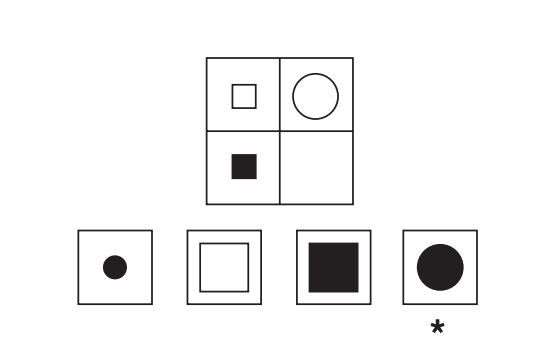
\includegraphics[width=0.5\linewidth]{image_pfc/Fig_9_8}
	\caption{在瑞文渐进矩阵测试中呈现给受试者的问题示例。
		受试者必须从底部的四个项目中选择一个,并将其放置在矩阵右下角单元格的缺失空间中。
		从左到右,形状变为圆形,但填充保持不变(白色)。
		因此,正如星号所标记的那样,正确的解决方案是在保持恒定填充(黑色)的情况下反映相同形状变化(正方形到圆形)的对象。
		转载自Duncan J.《智力是如何发生的》。©2010,耶鲁大学出版社,已获许可。\label{fig:fig_9_8}}
\end{figure}


当然,参加瑞文测试的人可以用文字来描述这种转变或关系。
但莱文等人(1982)描述了一个中风后失语的病人,据说他失去了所有的“内心语言”,也就是“听到”自己思考的感觉。
然而,他能解决雷文的问题,就像他这个年龄和职业的人所期望的那样。
所以这似乎是一个真正的非语言任务。


当人们执行瑞文的任务时,中外侧和腹侧前部皮层被激活(帕巴卡兰,1997)。
克里斯托夫等人(2001)声称,对于更困难的问题,激活的范围更大,延伸到极前部皮层的边界附近。
我们在本章的前面解释过,额极皮层的外侧部分可能是在猿人谱系中进化而来的。


邓肯(2000)使用了卡特尔的文化公平测试(卡特尔,1973),它类似于瑞文的渐进矩阵任务。
他们还发现中外侧前部皮层被激活,他们还发现空间和语言问题都会导致类似的激活。
患有前额叶或后顶叶病变的患者在这些测试中都有损伤,但患有颞叶病变的患者则没有(伍尔加,2010)。


所有这些问题都要求受试者对关系做出判断,类比也测试对关系的理解。
邦吉等人(2005)要求受试者说出“chain-link”是否类似于“bouquet-flower”。
当受试者做出这些判断时,前部皮层被激活,其峰值位于靠近额极皮层的边界。


随后的一项研究(文德尔肯,2008)使用了明确的类比,如“鞋子之于脚就像手套之于手”。
在一种情况下,受试者评估关系是否相似,这种情况鼓励受试者直接比较两个关系成分:鞋-脚和手套-手。
在这种情况下,激活发生在额极皮层外侧部分和中外侧前部皮层(46区)之间的边界附近。
在另一种情况下,受试者被要求提供“鞋子与脚的关系就像手套与脚的关系一样”,并需要提供“手”。
这种情况加重了语义检索,在这种情况下,激活发生在腹侧前部皮层。


我们建议用两种方法来解释这些激活。
首先,解决每个问题或类比需要在上下文的基础上生成目标。
在瑞文的任务中,前一两行提供了上下文。
其次,对上下文的分析需要对抽象规则的认识。
在较难的问题上,第一行和第二行各不相同,但它们遵循相同的抽象规则或关系。
然后,这个人必须通过将抽象规则应用于第三行中的项目来解决问题。
类比任务还涉及抽象的关系规则。
第 \ref{chap:chap3} - \ref{chap:chap8} 章反复论证灵长类动物的前皮层在通过抽象规则指导行为方面起着必要的作用。


通过一个特定的机制:再现。
根据这种观点,当被试判断" bouquet-flower "是否与" chain-link "相似时,他们必须比较两个明显不同的关系,为此,他们必须形成两个关系之间关系的表征,每个词对一个。
虽然我们认为类比和隐喻推理的能力可以被看作是层次结构的细化,它需要抽象规则的应用,但我们认识到需要更精确。
正如我们前面所说的,我们理解可以解释任何事情的模糊表述的危险。
因此,在结论部分,我们建议对第\ref{chap:chap8}章提出的基本功能进行阐述。



\textbf{总结}

我们认为,如第\ref{chap:chap8}章所述,前额叶皮层的基本功能可以被详细阐述以解释推理。
推理涉及根据抽象规则生成适合于复杂环境的目标。
随后,我们考虑在重新表征的背景下进行推理,并在人类前额叶皮层中添加新的层次。



\section{道德和社会规则}

最后,我们考虑一组不同的抽象规则,即适用于道德和社会行为的规则。
表\ref{tab:9_9}没有列出所有单独的激活,而是将它们全部作为了解或实现抽象规则的示例。
道德和社会规则是抽象的,因为它们适用于不同类型的行为。
道德或伦理规则规定一个人应该或不应该做什么。
社会规则决定了在特定的环境中什么行为是合适的。


道德教育教导人们在违反道德规则时通过批评自己来规范自己的行为(班杜拉,1997)。
因此,贝尔托斯等人(2006)在成年人考虑不同情况时对他们进行了扫描。
在一组条件中,受试者考虑他们故意违反社会规范的情况,例如在公共用餐期间将食物吐出来。
在其他条件下,他们考虑意外违反规范的情况,例如被食物呛到导致吐出来。
对比这些情况,贝尔托斯等人发现胼胝体吻侧至膝侧的内侧32区在大约相同的背腹侧水平上被激活。
他们还发现,与大脑皮层相连的杏仁核部分也被激活(贝克曼,2009)。


道德规范规范着社会生活,社会规范规范着交流与合作。
人类有公平和不公平交易的概念,最后通牒游戏探讨了公平的评估。
在这个任务中,一个人提出一个提议,另一个人可以拒绝或接受这个提议,但只能全盘接受。
在使用该任务的成像实验中,当受试者对不公平的提议做出反应时,激活发生在中外侧前部皮层、背扣带皮层和前岛皮层(三飞,2003)。
岛叶皮层的激活与拒绝不公平待遇有关,而中外侧前部皮层的激活与此无关。


\begin{table}[htbp] 
	\newcommand{\tabincell}[2]{\begin{tabular}{@{}#1@{}}#2\end{tabular}} %换行指令
	\centering
	\caption{人类大脑的激活\label{tab:9_9}}
	\renewcommand\arraystretch{1.5}	%设置表格内行间距
	\begin{tabular}{lll}
		\toprule
		详细阐述 & 激活 & 与基本函数的关系\\
		\midrule
		抽象的规则 & 代表道德和社会规则的 & 学习适合社会环境的规则  \\
		
		\bottomrule
		
	\end{tabular}%
\end{table}%


为了找出在执行这项任务时前额叶皮层的激活是否至关重要,诺奇等人(2006)在让受试者玩最后通牒游戏之前对他们进行了15分钟的rTMS。
在对右侧中外侧前部皮层进行破坏性刺激后,受试者对不公平提议的接受度增加。
另一方面,他们仍然认为这些提议不公平。


这种行为模式类似于双侧大面积前额叶皮层病变后的报道。


如前所述,双侧额叶较大病变的患者有时即使能准确地重复指示,也不能遵循指示。
邓肯等人(2008)将这种现象称为目标忽视。
我们将目标忽视归因于从长期记忆中检索规则的能力完好无损,以及在应用规则时在短期记忆中保持规则的能力受损。


与目标忽视类似的现象发生在腹内侧前额叶皮层和额极皮层病变的患者中。
克拉伊比奇等人(2009)在玩最后通牒游戏时研究了腹内侧和极侧前额皮质受损的患者。
病人提供的东西少了,内疚感也少了。
然而,当被问及其他人会怎么做时,他们知道适当的行为。
也就是说,他们知道社会规范,但他们没有遵守。


一个特别引人注目的案例来自一个名叫埃弗的病人,他接受了脑瘤手术。
患者双侧有很大的病变,包括腹侧前额叶皮层、眶额皮层和额极皮层,有时被称为“腹内侧前额叶皮层”病变。
请注意,在本书的其他地方,我们没有以这种不精确的方式使用术语腹内侧前额叶皮层。
赛风和达马西奥(1991)测试了埃弗对社会规范的了解,他似乎知道大多数这样的规则。
然而,在日常生活中,他未能履行自己的社会责任(埃斯林格和达马西奥,1985)。然而,埃弗从小就学会了这些规则和责任。
安德森等人(1999)描述了两名早期前额皮质受损的患者,成年后,这些患者在赛风和达马西奥(1991)用于社会规则知识的各种测试中表现不佳。


作为对这些损伤结果和成像实验结果的全面解释,福布斯和格拉夫曼(2010)提出,前叶皮层介导了对社会事件的认识。
这些知识可以通过向受试者展示社会脚本来测试,受试者必须描述一系列社会事件或对这些事件做出判断。
克鲁格等人(2009)认为内侧前额皮质在这种判断中起着特别关键的作用。
当被试描述社会活动,发现社会事件的正确顺序,或发现不一致时,激活发生在内侧前部皮层。


激活和相关的损伤效应表明,前叶皮层与道德和社会判断有关。
当人们对这些事情做出判断时,他们关心的是在社会背景下,对自己或对他人来说,哪些选择是合适的或允许的。
有人可能会争辩说,这种选择以一种相对直接的方式反映了所提议的功能。
在社会认知中,一个人必须按照抽象的规则,产生一个与当前情境相适应的目标,才会产生期望的结果。


这本书没有广泛论述社会行为。
除了偶尔提到猴群大小或群内竞争(第\ref{chap:chap2}章),我们强调前叶皮层在觅食选择中的作用。
在这样做的过程中,我们遵循我们所知道的证据,而从猴子的病变、细胞活动或成像中得到的证据中,并没有多少涉及社会互动。
因此,我们大多数关于人类前额皮质激活的讨论都遵循同样的思路。
然而,我们并不是说,前皮层的功能仅限于觅食选择。
社会选择涉及与觅食选择类似的机制,比如识别环境、产生适当的目标,并在记忆中保持这些目标。
然而,我们认识到,这些概念并不能说明社会行为中所有重要的方面。


随着人类社会系统的进化,它呈现出成像实验尚未探索的复杂性。


在他们的进化过程中,早期人类通过相互合作来适应,例如他们在狩猎大型动物时所做的(纵梁,2011)。
他们的生存依赖于群体生活,群体在不太积极的互动中从事贸易和交换(里德利,2010)。
人类社会也包括群体内部和群体之间的激烈竞争。
道德和社会行为比在成像实验中研究的任何东西都要复杂,因此我们并不认为情境、目标产生和在记忆中保持目标等概念深入研究了这个问题。



\section{结论}

本章探讨了第\ref{chap:chap8}章提出的建议是否可以解释复杂认知任务中的成像激活,并考虑了如何在人脑中阐述前额叶皮层的基本功能。


本章第一部分的解剖学回顾表明,与人类与猴子或黑猩猩的最后共同祖先相比,人类前皮层存在新的特征。
我们回顾了在原始人进化过程中颗粒状前额叶皮层扩张和形状改变的证据。
这种发展产生了几个后果。


1. 当前皮层与新皮层的比例增加时,更多的皮层可用于表征和再表征信息。


2. 前皮层的大小和细胞的树突棘密度影响信息被其细胞整合的程度。


3.白质体积的增加,其中包含连接一个前额叶皮层到另一个前额叶皮层的纤维,允许更大程度的跨域映射。


我们还提出了一些具有启发性的证据,表明随着现有区域的扩展,新的区域出现了。
如果是这样,那么这些新领域可能会在第\ref{chap:chap8}章描述的背景、目标和结果层次结构中添加进一步的层次。
这一发展可以看作是早期将第一个颗粒区域添加到大脑的过程的延续类人猿进化过程中灵长类和其他颗粒状前额叶皮层(第\ref{chap:chap2}章)。
我们使用了精化这个词来描述这些变化,这些变化有一个潜在的结果,即新的、更高的层次可以重新表示较低层次所表示的信息。
第\ref{chap:chap8}章解释了分层处理如何导致特征的抽象,我们认为重新表示需要相当程度的抽象。


本章的第二部分解释了第\ref{chap:chap8}章提出的建议如何解释当人们执行复杂任务时发生的成像激活认知任务。
为了方便读者,我们将本章中出现的表9.1-9.9编译成表\ref{tab:9_10}。
我们必须只包括数千个报告的激活的样本,但我们认为这些是那些在认知心理学家中有影响力的代表。
表\ref{tab:9_10}为这些激活分配了一个字母和数字,以备将来参考。


\begin{table}[htbp] 
	\newcommand{\tabincell}[2]{\begin{tabular}{@{}#1@{}}#2\end{tabular}} %换行指令
	\centering
	\caption{人类大脑的激活\label{tab:9_10}}
	\renewcommand\arraystretch{1.5}	%设置表格内行间距
	\begin{tabular}{lll}
		\toprule
		详细阐述 & 激活 & 与基本函数的关系\\
		\midrule
		环境 & C1 感觉决策 & 识别上下文  \\
		& C2 感官意象 & 产生感官情境 \\
		& C3 感官知觉 & 再现感官环境 \\
		目标 & G1 动词生成 & 根据上下文生成目标项  \\
		& G2 想象行动 & 生成适合上下文的目标 \\
		& G3 计划 & 生成目标序列 \\
		& G4 在内存中维护任务规则 & 任务规则的预期内存 \\
		& G5 在内存中维护未来任务 & 用于未来任务的前瞻性内存 \\
		& G6 监测自己的意图 & 采取行动 \\
		& G7 监视他人的意图 & 用手势预测他人的行为 \\
		结果 & O1 监控内部状态 & 评估结果  \\
		& O2 监测结果 & 评估结果 \\
		& O3 监控自己 & 再现自己行为的结果 \\
		将目标映射到上下文 & M1 言语配对联想 & 将提示词映射到响应词  \\
		& M2 单词含义 & 任意地将一个词映射到一个指涉 \\
		& M3 语义知识 & 关联表示,分类 \\
		从事件中生成目标 & E1 从记忆中检索事件& 检索情景记忆  \\
		& E2 想象未来事件 & 从情景记忆中产生事件 \\
		& E3 源内存 & 从关联项生成上下文 \\
		抽象的规则  & R1 推理 & 学习规则并应用于新问题  \\
		& R2 代表道德和社会规则 & 学习适合社会环境的规则 \\

		\bottomrule
		
	\end{tabular}%
\end{table}%


首先,为了方便读者,我们以其详细的形式重申第\ref{chap:chap8}章的建议:颗粒状前部皮层的基本功能,作为一个整体,是产生目标-作为行动目标的物体和地点-在当前环境和期望的结果中是适当的,根据当前的生物需求进行评估。
与系统发育上较老的学习系统相比,它可以基于单个事件专心地学习。
因此,它提供了一种减少错误的机制,它通过两种方式做到这一点:通过快速学习,以及通过提供一种学习和应用抽象规则和策略的机制。
必要时,前脑皮层在前瞻记忆中保存目标和目标序列,直到可以尝试实现它们。
在本章的前面,我们介绍了这个提议如何解释表9.10列出的许多激活。


1. 颗粒状前部皮层产生目标和目标序列。
当人们产生单词(G1)、想象物体(C2)、想象动作(G2)或想象未来动作(计划)(G3)时,颗粒状的前额叶皮层就会被激活。


2.颗粒状的前额叶皮层会有意识地而不是自动地产生目标。
当人们关注自己的意图时,颗粒状前部皮层就会被激活(G6)。


3.目标是适合当前环境的。当人们表示上下文(C1)、将反应词映射到提示词(M1)、将词映射到指代物(M2)、将物体映射到地点(M3)时,颗粒状前部皮层就会被激活。
在映射中,上下文充当先行词,目标充当后继词,这样上下文就映射到目标。


4. 这些目标适合于期望的结果和当前的需要。
当人们关注自己的生理需求(O1)和监测结果(O2)时,颗粒状前部皮层会发生激活。


5. 前额叶皮层可以在单一事件的基础上产生目标。
当人们检索情景记忆(E1)或检索情景记忆(E3)中与事件相关的上下文时,颗粒状前额叶皮层会被激活。


6. 前额叶皮层可以维持前瞻记忆中的目标。
当人们在记忆中保持当前(G4)或未来(G5)目标时,颗粒状前部皮层就会被激活。


我们认为,刚才列出的激活以一种相对直接的方式遵循我们的建议。
然而,颗粒状前部皮层的其他激活值得更多的评论。
这些激活与感官意识(C3)、解读他人的心理状态(G7)、自我监控(O3)、推理(R1)、表现或执行道德和社会规则(R2)以及想象未来事件(场景)(E2)有关。


我们的建议不能直接解释人类认知的这些方面,这并不奇怪。
第\ref{chap:chap8}章提出的建议取决于对类人猿进化和现代猴子前额叶皮层功能的看法。
理解意识、心智理论、自我评价、类比和隐喻推理、道德行为和想象场景依赖于对人类的研究。
我们已经提到,为了解释与这些概念相关的激活,我们诉诸于再现的概念。
然而,我们承认这样做的危险性,即我们可以如此随意地引用这个概念,以至于我们可以解释任何事情。
因此,为了限制我们的解释,我们要求将再现的解释与我们所描述的激活的特定位置联系起来,并将其与前脑皮层的整体组织联系起来。



\subsection{再描述}

为了说明我们的方法,我们首先考虑感官意识的激活(C3)。
罗和罗森塔尔(2011)讨论了意识的实证研究,并具体比较了主体的高阶和低阶观点。
在支持高阶观点的过程中,他们认为知觉涉及到低阶感官表征的表征。
正如第\ref{chap:chap7}章所述,我们知道关于物体的感觉信息到达中外侧和腹侧前部皮层,我们知道当受试者决定刺激是房子还是脸时,这些区域会发生激活(希克伦,2004)。
所以我们期望这些感官表征的再现发生在这些区域。
事实上,在罗和罗森塔尔(2006)的研究中,中外侧前部皮层的激活与受试者是否看到一个形状的报告有关。
这种激活涉及到“看见”的表象。



如果所有其他与意识相关的激活都发生在同一个地方,那么激活的位置就不重要了。
但事实并非如此。如果激活与自我意识(O1,O2和O3)有关,那么它们可以在内侧前部皮层找到。
这个发现是有原因的。正如我们在第\ref{chap:chap3}章中解释的那样,内侧前部皮层专门处理“内部”信号,而其他更外侧的前部皮层专门处理外部信号(罗森塔尔,2010)。


在再现的概念背后还有一个进一步的假设。
重新表征通过分层处理发生(第\ref{chap:chap8}章),高阶表征在分层中更明显地发生。
图\ref{fig:fig_9_7}所示的尾-吻侧梯度说明了这种层次结构,其中高阶表示(O3)位于低阶表示(O1)的吻侧。
正如刘和罗森塔尔(2011)所说,“自我参照意识思维依赖于三阶表征”。三阶表征指的是再表征的再表征。
二阶表征仅仅是表征的再表征。


我们现在可以把这些概念应用到推理(R1)中。
正如我们之前提到的,邦吉等人(2005)要求受试者说出“chain-link”是否类似于“bouquet-flower”。
主体有两个关系:“链环”和“花束”。
但是为了解决这个问题,他们必须比较这两种关系。
换句话说,它们必须代表两个关系之间的关系。
在这个实验中,激活发生在颗粒状前部皮层的吻侧部分,靠近额极皮层皮层和中外侧前部皮层的边界。
这个有问题的区域可能对应于46区或10区的吻侧部分,但无论精确位置如何,它似乎位于前额叶层级的较高位置。
它位于大脑半球的外侧表面,而不是内侧前部皮层,这可能反映了侧前部区域分析物体之间关系的低阶表征的事实。


与道德和社会规则(R2)相关的激活与刚才提到的不同,它们发生在中间表面。
我们看待吻侧和尾侧激活位点之间的关系的方式与刚才解释关系再现的方式大致相同。
更多的吻侧区域重新代表内侧额叶皮层更多尾部部分分析的信息。
正如第\ref{chap:chap3}章所解释的那样,这些区域分析行动的结果,专门研究“内部”信号。


首先,孩子们通过外部施加的制裁,比如惩罚,来学习道德和社会规则。
这就要求他们了解行动的结果。
但社会化的目的是教孩子内化规则,以规范自己的行为(班杜拉,2001)。
因此,当孩子们学习道德和社会规则时,“内部”信号变得越来越重要。
这就是为什么当成年人考虑他们故意藐视社会规范的情况时,激活发生在副扣带皮层(贝尔托斯,2006)。
这种激活位于胼胝体膝背腹侧的内侧32区,可以反映出调节自己行为的内疚感。
这可以从把自己描绘成一个遵守社会规则,行为道德的人开始。
当被试考虑诸如“好”或“善良”之类的特征性词汇是否适用于自己时,激活发生在几乎相同的区域,这一事实为这些观点提供了一些支持。
这个函数类似于前面提出的关系间关系的函数。
这里的再现也涉及到两个关系之间的关系。
一个涉及行为与道德或社会规范之间的关系,另一个涉及自我与道德或社会规范之间的关系。


\subsection{减少和避免错误}

我们故意把与想象未来事件有关的激活留到最后,也就是所谓的情景(E2)。
我们之前提到过,这些激活在解剖学上与人们回忆自传体记忆时发生的激活非常接近(哈萨比斯,2007)。
当人们想象未来的事件时,他们可以考虑假设的行动方案的结果。
换句话说,他们可以进行心理试错行为。
当人们想象未来事件时,激活发生在极前部皮层(哈萨比斯,2007),当受试者考虑备选选择(哈萨比斯,2009)和备选选择的相对价值(哈萨比斯,2009)时,该区域也会被激活。


我们在提案中说过,前叶皮质调节快速学习。
在类人猿的例子中,我们认为颗粒状前额叶皮层允许它们在一次试验中极限地学习(第\ref{chap:chap8}章)。
快速学习减少了猴子在适应新环境时出现的错误。
猴子也学习抽象的规则和策略,使它们能够像人类的前额叶皮层一样:限制错误,而不需要任何额外的学习,或者更常见的情况是,当它们把自己的快速学习机制用于解决问题时。
同样,基于单一事件在选择和结果之间分配因果责任的能力减少了未来的错误(第\ref{chap:chap4}章)。
因此,我们在第\ref{chap:chap8}章中提出,前部皮层赋予的优势涉及减少错误。
考虑到人们可以在想象中模拟行动,原则上,他们可以制定一个完全避免错误的计划。


还有其他方法可以让人们不犯错误地学习。
首先,他们可以根据口头指令行事,并且可以通过被告知的方式学习有关世界的事实。
阅读在视觉形态上也起到同样的作用。
我们回顾了一些证据,表明当人们准备按照任务指示行事时,以及当他们学习新知识时,颗粒状前部皮层会被激活。
第二,人们也可以通过模仿他人来学习,当他们能够辨别他人的意图时,这种行为就变得很重要。
我们已经证明,当人们模仿他人时,比如制作石器时,前额叶皮层会被激活。
当人们读懂别人的意图时,前脑皮层也会被激活。


第\ref{chap:chap8}章解释了灵长类动物前额叶皮层介导的进步减少了祖先强化学习机制中固有的错误。
因此,灵长类动物从它们的非灵长类祖先使用的缓慢的试错学习进化而来。
这些旧的学习系统通过对许多反馈事件进行平均来减少错误。
第\ref{chap:chap8}章认为,灵长类动物进化出了一种减少错误的能力,通过使用单一事件来产生目标,并在必要时对它们进行前瞻性编码,直到采取行动的时候。
在本章中,我们认为,在我们的进化过程中,人类将错误减少提高到一个新的水平。
人们可以从指导、模仿和心理试错行为中学习。
我们的祖先以某种方式克服了身体试错行为的需要,从而减少了随之而来的风险和不可避免的失败。
模仿和指导可以防止错误,只要某个问题的解决方案是群体中的一个成员所知道的。
但心理试错的作用不止于此。试错行为,完全在想象中进行,允许发展替代方案,完成潜在的结果。
人们可以尝试解决问题的不同方法,利用不同的知识领域,而不会产生任何风险,也不会浪费太多精力。
当与再现相结合时,这种认知操作变得更加强大。
当这些能力在人类进化过程中出现时,由精神时间旅行产生的场景允许人们在想象中发挥潜在的计划。
他们过去这样做的知识部分依赖于前脑皮层的再现。
通过这种方式,心理试错不仅可以减少错误,还可以提供洞察力。

